    \documentclass[xcolor=x11names]{beamer}
%%%%%%%%%%%%%%%%%%%%%%%%%%%%%%%%%%%%%%%%%%%%%%%%%%%%%%%%%%%%
%%  This Beamer template was created by Cameron Bracken.
%%  Anyone can freely use or modify it for any purpose
%%  without attribution.
%%
%%  Last Modified by C. Bracken: January 9, 2009
%%
%%  The preamble, and maybe some modification of the Cameron Bracken's template is due to Attila Molnár.
%%
%%

%% General document
\usepackage[utf8]{inputenc}
\usepackage[T1]{fontenc}
\usepackage{graphicx}
\usepackage{tikz}
\usetikzlibrary{decorations.fractals}
\usetikzlibrary{decorations.text}
\usepgflibrary{arrows}
\usetikzlibrary{fadings}
\usetikzlibrary[decorations.pathmorphing]
\tikzfading[name=fade inside, inner color=transparent!70, outer color=transparent!70]
\usetikzlibrary{calc}
\usetikzlibrary{intersections}
\usetikzlibrary{shapes}
\usetikzlibrary{patterns}
\usefonttheme{serif}
\usepackage{amssymb} 			
\usepackage{amsmath}
\usepackage{ifthen}
\usepackage[normalem]{ulem}
\usepackage{mathrsfs}

%%%%%%%%%%%%%%%%%%%%%%%%%%%%%%%%%%%%%%%%%%%%%%%%%%%%%%%%%%%%%%%%%%%%%%%%%%%%%%%%%%%%
%% Beamer Layout %%%%%%%%%%%%%%%%%%%%%%%%%%%%%%%%%%
\useoutertheme[subsection=false,shadow]{miniframes}
\useinnertheme{default}
\usefonttheme{serif}
%\usepackage{txfonts} %Hook for strict implication!
\DeclareSymbolFont{symbolsC}{U}{txsyc}{m}{n}
\DeclareMathSymbol{\strictif}{\mathrel}{symbolsC}{74}
\DeclareMathSymbol{\boxright}{\mathrel}{symbolsC}{128}
\usepackage{palatino}
%\usepackage[uppercase=upright,charter]{mathdesign}

\setbeamerfont{title like}{shape=\scshape}
\setbeamerfont{frametitle}{shape=\scshape}


\setbeamercolor*{lower separation line head}{bg=white!40!DeepSkyBlue3}
\setbeamercolor*{normal text}{fg=black,bg=white}
\setbeamercolor*{alerted text}{fg=red}
\setbeamercolor*{example text}{fg=black}
\setbeamercolor*{structure}{fg=black}

\setbeamercolor*{palette tertiary}{fg=black,bg=white!90!DeepSkyBlue3}
\setbeamercolor*{palette quaternary}{fg=black,bg=black!10}

%\setbeamercolor{block body alerted}{bg=normal text.bg!90!DeepSkyBlue4}
\setbeamercolor{block body}{bg=normal text.bg!95!DeepSkyBlue3}
%\setbeamercolor{block body example}{bg=normal text.bg!90!DeepSkyBlue4}
%\setbeamercolor{block title alerted}{use={normal text,alerted text},fg=alerted text.fg!75!normal text.fg,bg=normal text.bg!90!DeepSkyBlue4}
\setbeamercolor{block title}{bg=normal text.bg!70!DeepSkyBlue3}
%\setbeamercolor{block title example}{use={normal text,example text},fg=example text.fg!75!normal text.fg,bg=normal text.bg!75!DeepSkyBlue4}

\setbeamertemplate{blocks}[rounded][shadow=true]
%\setbeamertemplate{background canvas}[vertical shading][bottom=white,top=structure.fg!25]
%\setbeamertemplate{sidebar canvas left}[horizontal shading][left=white!40!black,right=black]
\setbeamertemplate{itemize items}[circle]
\setbeamercolor*{itemize item}{fg=DeepSkyBlue3}
\setbeamercolor*{itemize subitem}{fg=DeepSkyBlue3}
\setbeamercolor*{itemize subsubitem}{fg=DeepSkyBlue3}
\setbeamertemplate{enumerate items}[circle]
%\setbeamercolor{item projected}{bg=DeepSkyBlue3,fg=black}
\setbeamercolor{item projected}{bg=white,fg=DeepSkyBlue3}
\setbeamercolor*{enumerate item}{fg=DeepSkyBlue3}
\setbeamercolor*{enumerate subitem}{fg=DeepSkyBlue3}
\setbeamercolor*{enumerate subsubitem}{fg=DeepSkyBlue3}

%%%%%%%%%%%%%%%%%%%%%%%%%%%%%%%%%%%%%%%%%%%%%%%%%%


%%%%%%%%%%%%%%%%%%%%%%%%%%%%%%%%%%%%%%%%%%%%%%%%%%%%%%%%%%%%%%%%%%%%%%%%%%%%%%%%%%%%

\newenvironment{defi}[1][]{\begin{block}{\footnotesize \textsc{Definition} \ifthenelse{\equal{#1}{}}{}{\, (#1)}}}{\end{block}}
\newenvironment{prop}[1][]{\begin{block}{\footnotesize \textsc{Proposition} \ifthenelse{\equal{#1}{}}{}{\, (\textsc{#1})}}}{\end{block}}
\newenvironment{lemm}[1][]{\begin{block}{\footnotesize \textsc{Lemma} \ifthenelse{\equal{#1}{}}{}{\, (\textsc{#1})}}}{\end{block}}
\newenvironment{idea}[1][]{\begin{block}{\footnotesize \textsc{Idea} \ifthenelse{\equal{#1}{}}{}{\, (\textsc{#1})}}}{\end{block}}
\newenvironment{rema}[1][]{\begin{block}{\footnotesize \textsc{Remark} \ifthenelse{\equal{#1}{}}{}{\, (\textsc{#1})}}}{\end{block}}
\newenvironment{coro}[1][]{\begin{block}{\footnotesize \textsc{Corollary} \ifthenelse{\equal{#1}{}}{}{\, (\textsc{#1})}}}{\end{block}}
\newenvironment{tete}[1][]{\begin{block}{\footnotesize \textsc{Theorem} \ifthenelse{\equal{#1}{}}{}{\, (\textsc{#1})}}}{\end{block}}
\newenvironment{claim}[1][]{\begin{block}{Claim \ifthenelse{\equal{#1}{}}{}{\, (\textsc{#1})}}}{\end{block}}
%\newenvironment{lemma}[1][]{\begin{block}{Lemma \ifthenelse{\equal{#1}{}}{}{\, (\textsc{#1})}}}{\end{block}}
\newenvironment{question}[1][]{\begin{block}{Question \ifthenelse{\equal{#1}{}}{}{\, (\textsc{#1})}}}{\end{block}}
\newenvironment{rem}[1][]{\begin{block}{Remark \ifthenelse{\equal{#1}{}}{}{\, (\textsc{#1})}}}{\end{block}}
\newenvironment{homework}[1][]{\begin{block}{Homework \ifthenelse{\equal{#1}{}}{}{\, (\textsc{#1})}}}{\end{block}}
\newenvironment{proo}[1][]{\begin{block}{\footnotesize \textsc{Proof} \ifthenelse{\equal{#1}{}}{}{\, (\textsc{#1})}}}{\end{block}}

%%%%%%%%%%%%%%%%%%%%%
%% To evade unnecessary circles, mainly for \cimdia
%%%%%%%%%%%%%%%%%%%%%

\makeatletter
\let\beamer@writeslidentry@miniframeson=\beamer@writeslidentry
\def\beamer@writeslidentry@miniframesoff{%
  \expandafter\beamer@ifempty\expandafter{\beamer@framestartpage}{}% does not happen normally
  {%else
    % removed \addtocontents commands
    \clearpage\beamer@notesactions%
  }
}
\newcommand*{\miniframeson}{\let\beamer@writeslidentry=\beamer@writeslidentry@miniframeson}
\newcommand*{\miniframesoff}{\let\beamer@writeslidentry=\beamer@writeslidentry@miniframesoff}
\makeatother

%%%%%%%%%%%%%%%%%%%%%%%%%%%%%
%%%%%%%%%%%%% END %%%%%%%%%%%
%%%%%%%%%%%%%%%%%%%%%%%%%%%%%


%%%% Formatting Commands

\newcommand{\cimdia}[1] {\miniframesoff \begin{frame}\begin{center}\huge \begin{tabular}{c}#1\end{tabular}\end{center}\end{frame}\miniframeson}
\newcommand{\szakasz}[2][]{\section{#1}\subsection{}\cimdia{#2}}
\newcommand{\bluebullet}{\textcolor{DeepSkyBlue3}{\quad $\bullet$} \,\,}

\newenvironment{frame*}[1][]{\miniframesoff \begin{frame} #1}{\end{frame}\miniframeson}

  % for admissible intersections
  \newcommand{\bigsqcap}{\rotatebox[origin=c]{180}{$\bigsqcup$}}

\newcommand{\felkorvonal}[2]{\draw[rounded corners=0] (180+#1:.25*#2 cm) arc (180+#1:360+#1:.25*#2 cm)--cycle;}
\newcommand{\pecset}[2]{\begin{tikzpicture}[remember picture,overlay]
\node [ draw=red, rectangle, rounded corners=5mm, inner sep=1mm, ultra thick, fill=white, fill opacity=.8, rotate=30, scale=#1, text opacity=0.7] at (current page.center) {#2};\end{tikzpicture}}

\newcommand{\felirat}[7][]{\begin{tikzpicture}[remember picture,overlay]
\node [draw=DeepSkyBlue3, rectangle, rounded corners=#3 mm, inner sep=#2mm, ultra thick, fill=white, fill opacity=.8, scale=#4, text opacity=1,#1]
at ([xshift=#5 cm, yshift=#6 cm]current page.center) {#7};
\end{tikzpicture}}

\newcommand{\hazi}[6]{\begin{tikzpicture}[remember picture,overlay]
\node [ draw=Coral1,
        rectangle,
        rounded corners=#2 mm,
        inner sep=#1mm,
        ultra thick,
        fill=white,
        fill opacity=.8,
        rotate=0,
        scale=#3,
        text opacity=1]
        at ([xshift=#4 cm, yshift=#5 cm]current page.center)
        {#6};
\end{tikzpicture}}

\newcommand{\underconstruction}[1]{\begin{tikzpicture}[remember picture,overlay]
\node [rectangle, rounded corners=5mm, inner sep=1mm, rotate=30, scale=#1, text opacity=0.4]at (current page.center){\textsc{\textcolor{orange}{\begin{tabular}{c}under \\construction\end{tabular}}}};
\end{tikzpicture}}

\newcommand{\dzsa}[1]{\textsc{\underline{#1}}:}
\newcommand{\axiom}[1]{\bemph{(\mathrm{#1})}}



% Emphasizing:
\definecolor{barna}{rgb}{0.5,0.2,0.1}
\newcommand{\bemph}[1] {{\color{DeepSkyBlue3}{#1}}}
\newcommand{\kemph}[1] {{\color{blue}{#1}}}
\newcommand{\cemph}[1]{\textcolor{red}{#1}}
\newcommand{\zemph}[1] {{\color{Green2}{#1}}}
\newcommand{\yemph}[1] {{\color{Orange1}{#1}}}
%\renewcommand{\emph}[1]{\textbf{#1}}

\newcommand{\FD}{\mathbf F}
\newcommand{\FB}{\mathbf G}
\newcommand{\PD}{\mathbf P}
\newcommand{\PB}{\mathbf H}
\newcommand{\GB}{\mathbf A}
\newcommand{\GD}{\mathbf E}

\newcommand{\Pmodels}{\mathrel{\models \hspace{-1.8ex} \raisebox{1.1ex}{\scalebox{.5}{$\mathrm{\bemph{P}}$}} }\,}
\newcommand{\Omodels}{\mathrel{\models \hspace{-1.8ex} \raisebox{1.1ex}{\scalebox{.5}{$\mathrm{\bemph{O}}$}} }\,}
\newcommand{\Kmodels}{\mathrel{\models \hspace{-1.8ex} \raisebox{1.1ex}{\scalebox{.5}{$\mathrm{\bemph{K}}$}} }\,}
\newcommand{\Bmodels}{\mathrel{\models \hspace{-1.8ex} \raisebox{1.1ex}{\scalebox{.5}{$\mathrm{\bemph{B}}$}} }\,}
\newcommand{\tru}{\textup{true}}
\newcommand{\fal}{\textup{false}}
\newcommand{\und}{\textup{undefined}}


\newcommand{\FDDot}{\underline{\mathbf F}}
\newcommand{\FBDot}{\underline{\mathbf G}}
\newcommand{\PDDot}{\underline{\mathbf P}}
\newcommand{\PBDot}{\underline{\mathbf H}}

\newcommand{\CFD}{\mathbf F^c}
\newcommand{\CFB}{\mathbf G^c}
\newcommand{\CPD}{\mathbf P^c}
\newcommand{\CPB}{\mathbf H^c}

\newcommand{\CFDDot}{\underline{\mathbf F^c}}
\newcommand{\CFBDot}{\underline{\mathbf G^c}}
\newcommand{\CPDDot}{\underline{\mathbf P^c}}
\newcommand{\CPBDot}{\underline{\mathbf H^c}}

\renewcommand{\Diamond}{\scalebox{.9}{\raisebox{-.4ex}{\rotatebox{45}{$\Box$}}}}

%causal
\newcommand{\past}{\succ}
\newcommand{\pasteq}{\succeq}
\newcommand{\future}{\prec}
\newcommand{\futureeq}{\preceq}
%lightlike
\newcommand{\llpast}{\nwarrow}
\newcommand{\llpasteq}{\underline\nwarrow}
\newcommand{\llfuture}{\nearrow}
\newcommand{\llfutureeq}{\mathop{\underline\nearrow}}
%timelike
\newcommand{\tlpast}{\gg}
\newcommand{\tlpasteq}{\underline \gg}
\newcommand{\tlfuture}{\ll}
\newcommand{\tlfutureeq}{\underline \ll}

\newcommand{\egyuttjar}{\mathop{\uparrow \uparrow}}
\newcommand{\Between}{\mathrm{B}}
\newcommand{\EqDist}{\equiv}
\newcommand{\ISCM}{\uparrow\equiv\uparrow}

 \newcommand{\vonal} [1][.2]{\hspace{#1cm} | \hspace{#1cm}}

 \newcommand{\lrule}[3][c]{\begin{array}{#1} #2  \\  \hline #3 \end{array}}
 \newcommand{\dlrule}[3][c]{\begin{array}{#1} #2  \\  \hline\hline #3 \end{array}}
 \newcommand{\dual}{\delta}

 \newcommand{\mono}{\rightarrowtail}
 \newcommand{\epi}{\twoheadrightarrow}
 \newcommand{\iso}{\rightarrowtail \!\!\!\!\! \rightarrow}

 \newcommand{\defegy}[1][.1]{\hspace{#1cm}\overset{\textup{\tiny def}}{=}\hspace{#1cm}}
 \newcommand{\defpont}[1][.1]{\hspace{#1cm}\overset{\textup{\tiny def}}{:}\hspace{#1cm}}
 \newcommand{\defekv}[1][.1]{\hspace{#1cm}\overset{\textup{\tiny def}}{ \Leftrightarrow }\hspace{#1cm}}
 \newcommand{\lthen}{\rightarrow}
 \newcommand{\liff}{\leftrightarrow}
 \newcommand{\forallin}[2]{(\forall #1 \in #2)}
 \newcommand{\existsin}[2]{(\exists #1 \in #2)}
 \newcommand{\nexistsin}[2]{(\nexists #1 \in #2)}
 \newcommand{\forallp}[1]{(\forall #1)}
 \newcommand{\existsp}[1]{(\exists #1)}

 \newcommand{\points}[1][0]{\hspace{#1ex}\hspace{-.5ex}:\hspace{-.5ex}\hspace{#1ex}}
 \newcommand{\Points}{\mathrm{P}}
 \newcommand{\Pointsf}{\mathrm{p}}
 \newcommand{\Ex}{\mathrm{E}}

\newcommand{\wline}[1]{\mathrm{wline}_{#1}}

\newcommand{\magyi}[1]{\textup{\bemph{\tiny #1}}}
\newcommand{\magyarazat}[2]{\overset{\substack{\textup{#2}\\ \downarrow}}{#1}}
\newcommand{\wintension}[3][]{{[}\hspace{-.46mm}{[} {#3}{]}\hspace{-.46mm}{]}^{\mathfrak{#1}}_{#2}}
\newcommand{\canintension}[2][]{{[}\hspace{-.46mm}{[} {#2}{]}\hspace{-.46mm}{]}_{\mathrm{#1}}}
\newcommand{\intension}[2][]{{[}\hspace{-.46mm}{[} {#2}{]}\hspace{-.46mm}{]}^{\mathfrak{#1}}}

\newcommand{\theory}[2][]{\mathrm{th}_{\mathfrak{#1}}(#2)}

\newcommand{\seenby}{\reflectbox {$R$}}
\newcommand{\derives}[1][]{\vdash_{\mathrm{#1}}}


\newcommand{\PBTemplate}[1]{{#1} \overrightarrow {\PB}}
\newcommand{\FBTemplate}[1]{{#1} \overrightarrow {\FB}}
\newcommand{\BoxTemplate}[1]{{#1} \overrightarrow {\Box}}
\newcommand{\PDTemplate}[1]{{#1} \widehat {\PD}}
\newcommand{\FDTemplate}[1]{{#1} \widehat {\FD}}
%\newcommand{\DiamondTemplate}[1]{#1\hspace{-.2ex} \mathop{\Diamond\hspace{-1.35ex} \raisebox{.4ex}{\scalebox{.5}{$\land$}}}\,}

%%%%%%%%%%%%%%%%%%%%%%%%%%%%%%%%%%%%%%%%%%%%%%%%%%%%%%
\newenvironment{tomb}[2][.1]{\arraycolsep=#1cm\begin{array}{#2}}{\end{array}}

\beamertemplatenavigationsymbolsempty

%%%%%%%%%%%%%%%%%%%%%%%%%%% COORDINATE SYSTEMS
% COORDSYS (ORIGOCOORDINATENAME, WIDTH, HEIGHT)
% Draws a Coordinatesystem around ORIGOCOORDINATENAME with a width of WIDTH and a height of HEIGHT,
% names the beginning and end of axes, southwest corner, northwest corner,
\newcommand{\CoordSys}[3]{
\coordinate (XY#1) at ([xshift=#2 cm, yshift=#3 cm]#1);
\coordinate (-XY#1) at ([xshift=-#2 cm, yshift=-#3 cm]#1);
\coordinate (-X#1) at ([xshift=-#2 cm]#1);
\coordinate (X#1) at ([xshift=#2 cm]#1);
\coordinate (Y#1) at ([yshift=#3 cm]#1);
\coordinate (-Y#1) at ([yshift=-#3 cm]#1);
\draw [help lines, step=.5cm] (-XY#1) grid (XY#1);
\draw[->] (-X#1)--(X#1);
\draw[->] (-Y#1)--(Y#1);
}

\newcommand{\OneQuadrantCoordSys}[3]{
\coordinate (XY#1) at ([xshift=#2 cm, yshift=#3 cm]#1);
%\coordinate (-XY#1) at ([xshift=-#2 cm, yshift=-#3 cm]#1);
%\coordinate (-X#1) at ([xshift=-#2 cm]#1);
\coordinate (X#1) at ([xshift=#2 cm]#1);
\coordinate (Y#1) at ([yshift=#3 cm]#1);
%\coordinate (-Y#1) at ([yshift=-#3 cm]#1);
%\draw [help lines, step=.5cm] (#1) grid (XY#1);
\draw[->, name path=XAxis#1] (#1)--(X#1);
\draw[->, name path=YAxis#1] (#1)--(Y#1);
}

% \DistanceLabel{SS}{AS}{-45}{1}{pos=.5}{1}
\newcommand{\DistanceLabel}[6]{
\coordinate(#1horgony) at ([shift=(#3:#4)] #1);
\coordinate(#2horgony) at ([shift=(#3:#4)] #2);
\draw[thin, red, <->] (#1horgony)--(#2horgony) node[#5, scale=.7]{#6};
\draw[opacity=.4, black] (#1)--(#1horgony);
\draw[opacity=.4, black] (#2)--(#2horgony);
}



%Lorentz(OriginalOriginCoord, ResultingOriginCoord, SpeedNum, PointCoord, Label)
%
\newcommand{\Lorentz}[5]{
\path (#1); \pgfgetlastxy{\XCoord}{\YCoord}; % Extracting coordinates of the Origin
\pgfmathsetmacro{\XOrigin}{\XCoord} % Saving X coordinate
\pgfmathsetmacro{\YOrigin}{\YCoord} % Saving Y coordinate
\path (#4); \pgfgetlastxy{\XCoord}{\YCoord}; % Extracting coordinates of the Point
\pgfmathsetmacro{\XEvent}{\XCoord} % Saving X coordinate
\pgfmathsetmacro{\YEvent}{\YCoord} % Saving Y coordinate
\pgfmathsetmacro{\XEventWRTOrigin}{\XEvent-\XOrigin} % Relativizing to the origin
\pgfmathsetmacro{\YEventWRTOrigin}{\YEvent-\YOrigin} % Relativizing to the origin
\pgfmathparse{XLorentz(#3,\XEventWRTOrigin,\YEventWRTOrigin)} % transforming x
\pgfmathsetmacro{\XEventTr}{\pgfmathresult} % save the result of x
\pgfmathparse{YLorentz(#3,\XEventWRTOrigin,\YEventWRTOrigin)} % transforming y
\pgfmathsetmacro{\YEventTr}{\pgfmathresult} % save the result of y
\node[world](#5) at (
[xshift=\XEventTr pt,
 yshift=\YEventTr pt] #2){};
}

\newcommand{\ThreeDimCoordSys}[4]{
\coordinate (XY#1) at ([xshift=#2 cm, yshift=#3 cm]#1);
\coordinate (-XY#1) at ([xshift=-#2 cm, yshift=-#3 cm]#1);
\coordinate (X#1) at ([xshift=#2 cm]#1);
\coordinate (-X#1) at ([xshift=-#2 cm]#1);
\coordinate (Y#1) at ([yshift=#3 cm]#1);
\coordinate (-Y#1) at ([yshift=-#3 cm]#1);
%\path (#1); \pgfgetlastxy{\XCoord}{\YCoord}; % Extracting coordinates of the Origin
%\pgfmathsetmacro{\XCoordcm}{\XCoord/28.4527}
%\pgfmathsetmacro{\YCoordcm}{\YCoord/28.4527}
%\coordinate (Z#1) at (\XCoordcm, \YCoordcm,#4);
%\coordinate (-Z#1) at (\XCoordcm, \YCoordcm,-#4);
%\draw [help lines, step=.5cm] (-XY#1) grid (XY#1);
\coordinate (Z#1) at ([shift=(\ThirdAxisAngle : #4*\ThirdAxisUnit cm)]#1);
\coordinate (-Z#1) at ([shift=(\ThirdAxisAngle : #4*\ThirdAxisUnit cm)]#1);
\draw[->, name path=XAxis#1] (#1)--(X#1);
\draw[->, name path=YAxis#1] (#1)--(Y#1);
\draw[->, name path=ZAxis#1] (#1)--(Z#1);
}


\newdimen\XCoord
\newdimen\YCoord




\author{Attila Moln\'ar}
\date{2014. March 21.}
\title{Test}
\institute{ELTE}
\begin{document}
\footnotesize



%%%%%%%%%%%%%%%%%%%%%%%%%%%%%%% SLIDE %%%%%%%%%%%%%%%%%%%%%%%%%%%%%%%%%%%%%%%%%%%%%
\begin{frame}
\frametitle{About some words}
\begin{itemize}
\item \textbf{Relativity}: things such as
 \begin{itemize}\footnotesize
 \item time of things
 \item length of things
 \item simultaneity of things
 \item mass (kinetic energy) of things
 \end{itemize}
 are \cemph{relative to the speed of the observer} since (Einstein 1905).
\item \textbf{Special Relativity}: Relativistic Physics in which acceleration and gravitation is ignored.
\item \textbf{General Relativity}: Relativistic Physics in which acceleration and/or gravitation is not ignored.
\item \textbf{Kinematics}: physics of moving (speed).
\item \textbf{Dynamics}: physics of collisions (mass).
\end{itemize}

\end{frame}
%%%%%%%%%%%%%%%%%%%%%%%%%%%%%%% SLIDE %%%%%%%%%%%%%%%%%%%%%%%%%%%%%%%%%%%%%%%%%%%%%
%%%%%%%%%%%%%%%%%%%%%%%%%%%%%%% SLIDE %%%%%%%%%%%%%%%%%%%%%%%%%%%%%%%%%%%%%%%%%%%%%
\szakasz[Intro]{Introduction into \\ Special Relativity}
\begin{frame}
\frametitle{Spacetime Diagrams}
\framesubtitle{Important events in the life of Alice and Bob}
\vspace{-.5cm}\[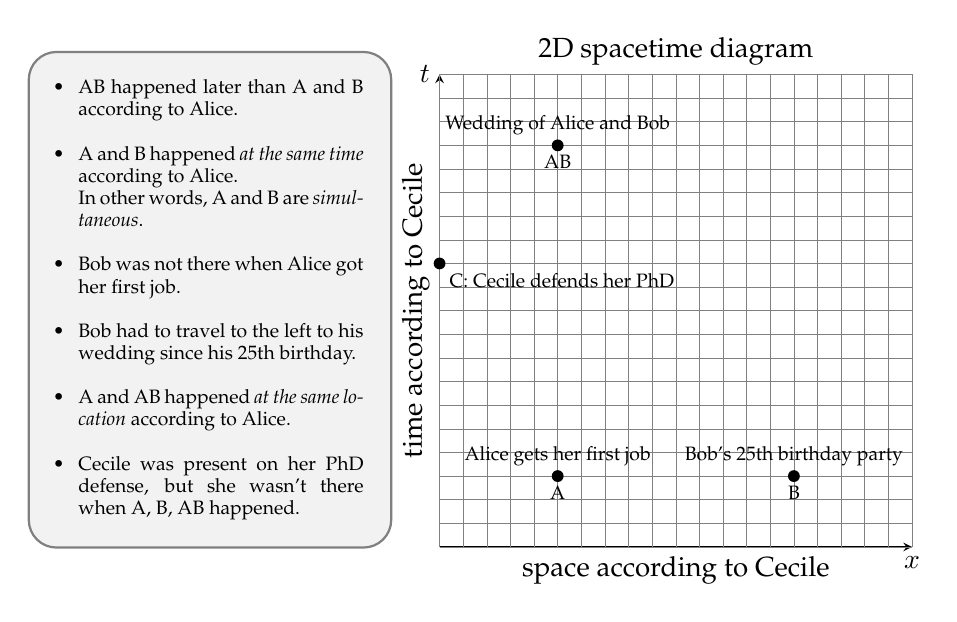
\begin{tikzpicture}[>=stealth, scale=.6,
world/.style={inner sep=0, minimum size=.15cm, fill=black, circle},
intension/.style={rounded corners=10pt, fill=white!90!gray, fill opacity=1, draw=gray, thick, inner sep=10},
altrel/.style={->},
axis/.style={->},
felirat/.style={inner sep=5, scale=.7},
bejaras/.style={blue}]
\node at (5,10.5) {2D spacetime diagram};
\coordinate (O) at (0,0);
\coordinate (Y) at (0,10);
\coordinate (X) at (10,0);
\draw[axis]  (O) -- (Y) node[midway, above, sloped]{time according to Cecile};
\draw[axis]  (O) -- (X) node[midway, below, sloped]{space according to Cecile};;
\node[anchor=north] at (X) {$x$};
\node[anchor=east] at (Y) {$t$};
\draw [help lines, step=.5cm] (O) grid (10,10);
%%%%%%%%%% PAUSE %%%%%%%%%%%
\node [world] (A) at (2.5,1.5) {};
\node [felirat, anchor=south] at (A) {Alice gets her first job};
\node [felirat, anchor=north] at (A) {A};
\node [world] (B) at (7.5,1.5) {};
\node [felirat, anchor=south] at (B) {Bob's 25th birthday party};
\node [felirat, anchor=north] at (B) {B};
\node [world] (C) at (2.5,8.5) {};
\node [felirat, anchor=south] at (C) {Wedding of Alice and Bob};
\node [felirat, anchor=north] at (C) {AB};
\node [world](Cec) at (0,6) {};
\node [felirat, anchor=north west] at (Cec) {C: Cecile defends her PhD};
%%%%%%%%%% PAUSE %%%%%%%%%%%
\node[anchor=north east, intension] at (-1,10.5) {\hspace{-.6cm}\begin{minipage}{4.5cm}
\scriptsize\begin{itemize}
\item AB happened later than A and B according to Alice.
\item A and B happened \emph{at the same time} according to Alice. \\ In other words, A and B are \emph{simultaneous}.
\item Bob was not there when Alice got her first job.
\item Bob had to travel to the left to his wedding since his 25th birthday.
\item A and AB happened \emph{at the same location} according to Alice.
\item Cecile was present on her PhD defense, but she wasn't there when A, B, AB happened.
\end{itemize}
\end{minipage}};
%%%%%%%%%% PAUSE %%%%%%%%%%%

\end{tikzpicture}\]\end{frame}
%%%%%%%%%%%%%%%%%%%%%%%%%%%%%%% SLIDE %%%%%%%%%%%%%%%%%%%%%%%%%%%%%%%%%%%%%%%%%%%%%
%%%%%%%%%%%%%%%%%%%%%%%%%%%%%%% SLIDE %%%%%%%%%%%%%%%%%%%%%%%%%%%%%%%%%%%%%%%%%%%%%
\begin{frame}
\frametitle{Spacetime Diagrams}
\framesubtitle{Randevous of Alice and Bob}
\vspace{-1cm}
\[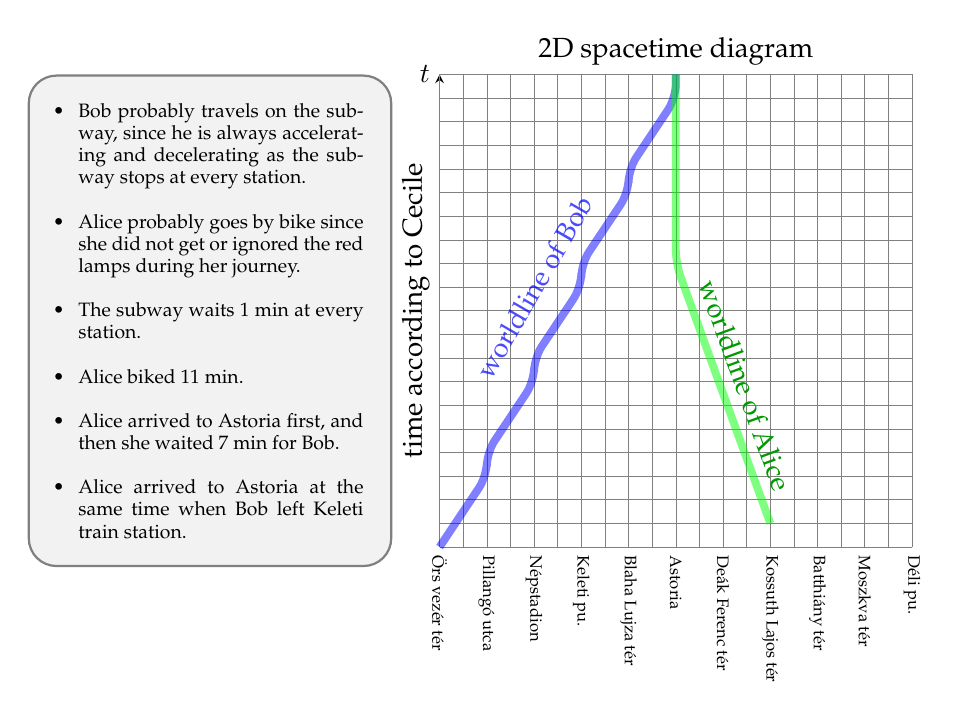
\begin{tikzpicture}[>=stealth, scale=.6,
world/.style={inner sep=0, minimum size=.15cm, fill=black, circle},
intension/.style={rounded corners=10pt, fill=white!90!gray, fill opacity=1, draw=gray, thick, inner sep=10},
altrel/.style={->},
worldline/.style={line width=1mm, rounded corners=5, opacity=.5},
axis/.style={->},
felirat/.style={inner sep=5, scale=.6},
bejaras/.style={blue}]
\node at (5,10.5) {2D spacetime diagram};
\coordinate (O) at (0,0);
\coordinate (Y) at (0,10);
\coordinate (X) at (10,0);
\draw[axis]  (O) -- (Y) node[midway, above, sloped]{time according to Cecile};
\node[anchor=north] at (X) {};%$x$};
\node[anchor=east] at (Y) {$t$};
\draw [help lines, step=.5cm] (O) grid (10,10);
\node[anchor=north east, intension] at (-1,10) {\hspace{-.6cm}\begin{minipage}{4.5cm}
\scriptsize\begin{itemize}
\item Bob probably travels on the subway, since he is always accelerating and decelerating as the subway stops at every station.
\item Alice probably goes by bike since she did not get or ignored the red lamps during her journey.
\item The subway waits 1 min at every station.
\item Alice biked 11 min.
\item Alice arrived to Astoria first, and then she waited 7 min for Bob.
\item Alice arrived to Astoria at the same time when Bob left Keleti train station.
\end{itemize}
\end{minipage}};
\coordinate (B1) at (0,0) {};
\coordinate (B2) at (1,1.5) {} {};
\coordinate (B3) at (1,2) {} {};
\coordinate (B4) at (2,3.5) {} {};
\coordinate (B5) at (2,4) {} {};
\coordinate (B6) at (3,5.5) {} {};
\coordinate (B7) at (3,6) {} {};
\coordinate (B8) at (4,7.5) {} {};
\coordinate (B9) at (4,8) {} {};
\coordinate (B10) at (5,9.5) {} {};
\coordinate (B11) at (5,10) {} {};
\coordinate (C1) at (7,0.5) {} {};
\coordinate (C2) at (5,6) {} {};
\node [felirat, anchor=west, rotate=-90] at (0,0) {Örs vezér tér};
\node [felirat, anchor=west, rotate=-90] at (1,0) {Pillangó utca};
\node [felirat, anchor=west, rotate=-90] at (2,0) {Népstadion};
\node [felirat, anchor=west, rotate=-90] at (3,0) {Keleti pu.};
\node [felirat, anchor=west, rotate=-90] at (4,0) {Blaha Lujza tér};
\node [felirat, anchor=west, rotate=-90] at (5,0) {Astoria};
\node [felirat, anchor=west, rotate=-90] at (6,0) {Deák Ferenc tér};
\node [felirat, anchor=west, rotate=-90] at (7,0) {Kossuth Lajos tér};
\node [felirat, anchor=west, rotate=-90] at (8,0) {Batthiány tér};
\node [felirat, anchor=west, rotate=-90] at (9,0) {Moszkva tér};
\node [felirat, anchor=west, rotate=-90] at (10,0) {Déli pu.};
\draw[worldline, blue] (B1)--(B2)--(B3)--(B4)--(B5)--(B6)--(B7)--(B8)--(B9)--(B10)--(B11);
\draw[worldline, green] (C1)--(C2) node[opacity=1, green!60!black, sloped, above,pos=.5]{worldline of Alice}--(B10)--(B11);
\node[blue, opacity=.7, rotate=60] at (2,5.5) {worldline of Bob};
\end{tikzpicture}\]\end{frame}
%%%%%%%%%%%%%%%%%%%%%%%%%%%%%%% SLIDE %%%%%%%%%%%%%%%%%%%%%%%%%%%%%%%%%%%%%%%%%%%%%
%%%%%%%%%%%%%%%%%%%%%%%%%%%%%%% SLIDE %%%%%%%%%%%%%%%%%%%%%%%%%%%%%%%%%%%%%%%%%%%%%
\begin{frame}
\vspace{-.55cm}
\[\hspace{-1cm}
\footnotesize
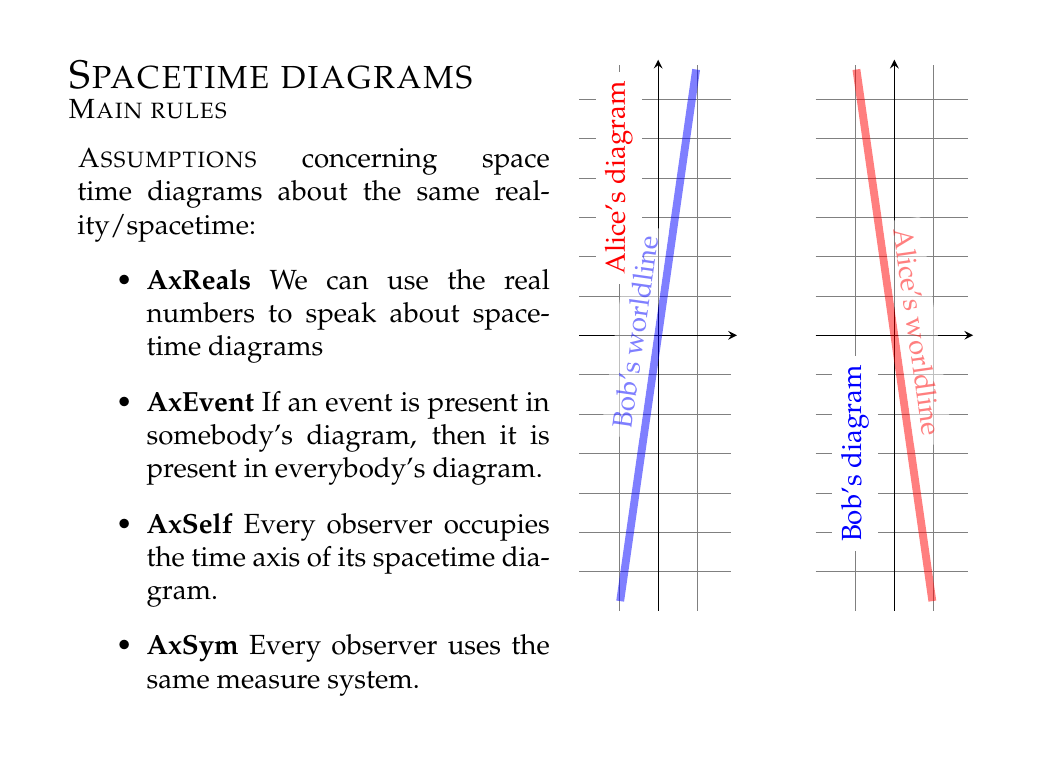
\begin{tikzpicture}[>=stealth, scale=1,
world/.style={inner sep=0, minimum size=.15cm, fill=black, circle},
intension/.style={rounded corners=10pt, fill=white!90!gray, fill opacity=1, draw=gray, thick, inner sep=10},
worldline/.style={line width=1mm, rounded corners=1pt, opacity=.5},
axis/.style={->},
felirat/.style={inner sep=5, scale=.7},
bejaras/.style={blue}]


% SLIDE TITLE
\node[anchor=north west, inner sep=0] at (0.5,8.5) {\textsc{\Large Spacetime diagrams}};
\node[anchor=north west, inner sep=0] at (0.5,8) {\textsc{\normalsize Main rules}};
% SIZE OF THE SLIDE
\draw[white]  (0,0) rectangle (12.77,8.9);
%%%%%%%%% TEXT %%%%%%%%%%%%%
\node[anchor=north west] at (0.5,7.5) {\begin{minipage}{6cm}
\textsc{Assumptions} concerning space time diagrams about the same reality/spacetime:
\begin{itemize}
%\item \textsc{Empirical fact}: The speed of light is the same for every observer.
\item \textbf{AxReals} We can use the real numbers to speak about spacetime diagrams
\item \textbf{AxEvent} If an event is present in somebody's diagram, then it is present in everybody's diagram.
\item \textbf{AxSelf} Every observer occupies the time axis of its spacetime diagram.
\item \textbf{AxSym} Every observer uses the same measure system.
\end{itemize}
\end{minipage}
};
%%%%%%%%%%%%%%%%%%%%%%%%%%%
% 1st COORDINATE SYSTEM
\coordinate (XY) at (9,8.5) {} {};
\coordinate (-XY) at (7,1.5) {} {} {};
\coordinate (-X) at (7,5) {} {} {} {};
\coordinate (X) at (9,5) {} {} {} {};
\coordinate (Y) at (8,8.5) {};
\coordinate (-Y) at (8,1.5) {} {} {};
\draw [help lines, step=.5cm] (-XY) grid ([shift=(-135:1mm)]XY);
\draw[->] (-X)--(X);
\draw[->] (-Y)--(Y);
\node(A1) at (7.5,1.5) {};
\node(A2) at (8.5,8.5) {};
%%%%%%%%%%%%%%%%%%%%%%%%%%
\begin{scope}[xshift=3cm]
\coordinate (2XY) at (9,8.5) {} {};
\coordinate (2-XY) at (7,1.5) {} {} {};
\coordinate (2-X) at (7,5) {} {} {} {};
\coordinate (2X) at (9,5) {} {} {} {};
\coordinate (2Y) at (8,8.5) {};
\coordinate (2-Y) at (8,1.5) {} {} {};
\draw [help lines, step=.5cm] (2-XY) grid ([shift=(-135:1mm)]2XY);
\draw[->] (2-X)--(2X);
\draw[->] (2-Y)--(2Y);
\node(2A1) at (8.5,1.5) {};
\node(2A2) at (7.5,8.5) {};
\end{scope}
\node[rotate=90, text=red, fill=white] at (7.5,7) {Alice's diagram};
\node[rotate=90, text=blue, fill=white]  at (10.5,3.5)  {Bob's diagram};
\draw[worldline, blue] (A1)--(A2) node[fill=white, sloped, above, pos=.5]{Bob's worldline};
\draw[worldline, red] (2A1)--(2A2) node[fill=white, sloped, above, pos=.5]{Alice's worldline};
\end{tikzpicture}\]
\end{frame}
%%%%%%%%%%%%%%%%%%%%%%%%%%%%%%% SLIDE %%%%%%%%%%%%%%%%%%%%%%%%%%%%%%%%%%%%%%%%%%%%%
\begin{frame}[fragile]
\vspace{-.55cm}
\[\hspace{-1cm}
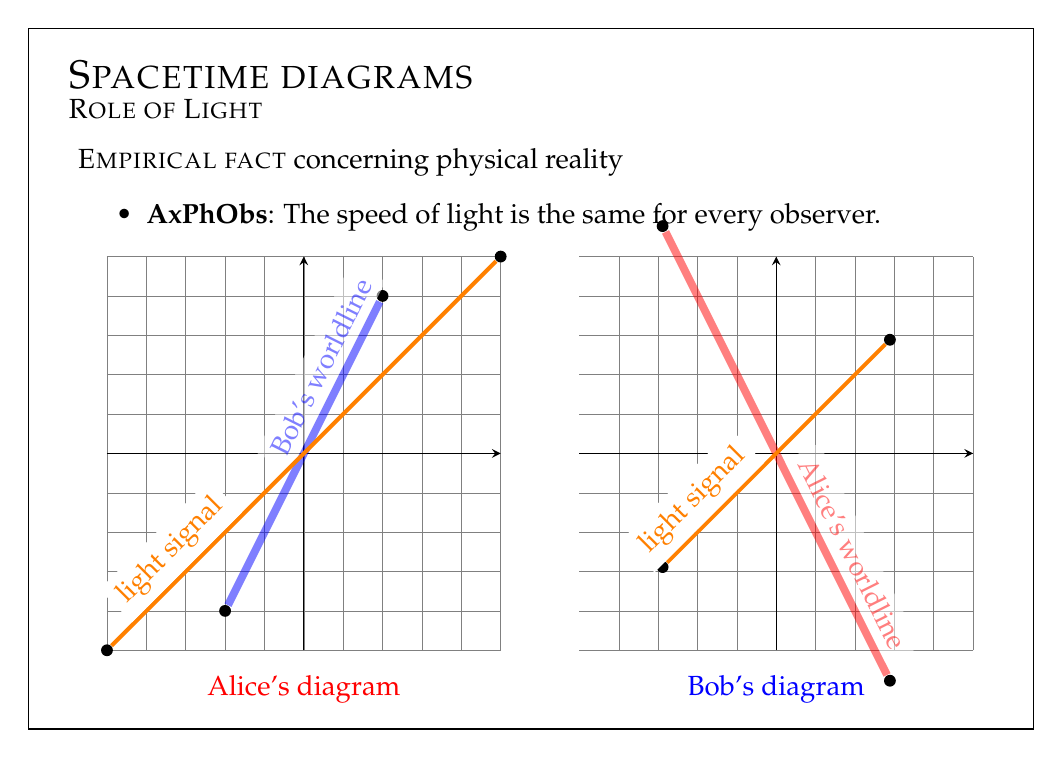
\begin{tikzpicture}[>=stealth, scale=1,
world/.style={inner sep=0, minimum size=.15cm, fill=black, circle},
worldline/.style={line width=1mm, rounded corners=1pt, opacity=.5},
axis/.style={->},
light/.style={orange, line width=.5mm}]
\pgfmathdeclarefunction{XLorentz}{3}{\pgfmathparse{(#2 - #1*#3)/(sqrt(1-(#1)^2))}} % speed, spacecoord, timecoord
\pgfmathdeclarefunction{YLorentz}{3}{\pgfmathparse{(#3 - #1*#2)/(sqrt(1-(#1)^2))}} % speed, spacecoord, timecoord
%%%%%%%%%%%%%%%%%%%%%%% DIA KEZDETE %%%%%%%%%%%%%%%%%%%%%%%%%%%
\node[anchor=north west, inner sep=0] at (0.5,8.5) {\textsc{\Large Spacetime diagrams}}; %%%%%%% TITLE
\node[anchor=north west, inner sep=0] at (0.5,8) {\textsc{\normalsize Role of Light}}; %%%%%%% SUBTITLE
\draw%[white]  %%%%%%%%%%%% SIZE OF THE SLIDE
      (0,0) rectangle (12.77,8.9);
%%%%%%%% TEXT %%%%%%%%%%%%%
\node[anchor=north west] at (0.5,7.5) {\begin{minipage}{12cm}
\textsc{Empirical fact} concerning physical reality
\begin{itemize}
\item \textbf{AxPhObs}: The speed of light is the same for every observer.
\end{itemize}
\end{minipage}
};
%%%%%%%%%%%%%%%%%%%%%%% KOORDINÁTARENDSZEREK %%%%%%%%%%%%%%%%%%%%%%%%%%%
\coordinate(O1) at (3.5,3.5);
  \CoordSys{O1}{2.5}{2.5}
\coordinate(O2) at (9.5,3.5);
  \CoordSys{O2}{2.5}{2.5}
%%%%%%%%%%%%%
% SETTINGS %%
%%%%%%%%%%%%%
\coordinate (SignalStart) at (1,1) {} {};
\coordinate (SignalBounced) at (6,6) {};
\coordinate (AliceStart) at (3.5,1) {};
\coordinate (AliceEnd) at (3.5,6) {};
\coordinate (BobStart) at (2.5,1.5) {} {} {}; % Fontos hogy átmenjen az Origón, különben rossz a lorentz transzformáció!!
\coordinate (BobEnd) at (4.5,5.5) {} {} {};
%%%%%%%%%% Ezt lehetne macronak, speedszámítócuccnak
\path (BobStart); \pgfgetlastxy{\XCoord}{\YCoord}; % Extracting coordinates of the Origin
\pgfmathsetmacro{\XFirst}{\XCoord} % Saving X coordinate
\pgfmathsetmacro{\YFirst}{\YCoord} % Saving Y coordinate
\path (BobEnd); \pgfgetlastxy{\XCoord}{\YCoord}; % Extracting coordinates of the Point
\pgfmathsetmacro{\XSecond}{\XCoord} % Saving X coordinate
\pgfmathsetmacro{\YSecond}{\YCoord} % Saving Y coordinate
\pgfmathsetmacro{\SpeedBob}{(\XFirst-\XSecond)/(\YFirst-\YSecond)} % Relativizing to the origin
%%%%%%%%%%%%%%%%%%%%%%%%%%%%%%%%%%
\Lorentz{O1}{O1}{0}{BobStart}{BS}
\Lorentz{O1}{O1}{0}{BobEnd}{BE}
\Lorentz{O1}{O1}{0}{SignalStart}{SS}
\Lorentz{O1}{O1}{0}{SignalBounced}{SB}
\Lorentz{O1}{O2}{\SpeedBob}{AliceStart}{AS'}
\Lorentz{O1}{O2}{\SpeedBob}{AliceEnd}{AE'}
\Lorentz{O1}{O2}{\SpeedBob}{SignalStart}{SS'}
\Lorentz{O1}{O2}{\SpeedBob}{SignalBounced}{SB'}
\node[rotate=0, text=red, fill=white] at (3.5,0.5) {Alice's diagram};
\node[rotate=0, text=blue, fill=white] at (9.5,0.5) {Bob's diagram};
\draw[worldline, blue] (BS)--(BE) node[fill=white, sloped, above, pos=.75]{Bob's worldline};
\draw[worldline, red] (AS')--(AE') node[fill=white, sloped, above, pos=.25]{Alice's worldline};
\draw[light]  (SS)-- (SB) node[fill=white, sloped, above, pos=.2]{light signal};
\draw[light]  (SS')-- (SB') node[fill=white, sloped, above, pos=.2]{light signal};
\end{tikzpicture}\]
\end{frame}
%%%%%%%%%%%%%%%%%%%%%%%%%%%%%% SLIDE %%%%%%%%%%%%%%%%%%%%%%%%%%%%%%%%%%%%%%%%%%%%%
\szakasz[Paradigmatic Effects]{Paradigmatic Relativistic Effects}
\begin{frame}
\frametitle{Paradigmatic Relativistic Effects}
\begin{itemize}
\item \textbf{Asynchron}: Moving pairs of clocks get out of synchronism
\item \textbf{Time Dilation}: Moving clocks slow down.
\item \textbf{Length Contraction}: Moving meter rods shrink.
\end{itemize}
\end{frame}
%%%%%%%%%%%%%%%%%%%%%%%%%%%%%% SLIDE %%%%%%%%%%%%%%%%%%%%%%%%%%%%%%%%%%%%%%%%%%%%%
\begin{frame}[fragile]
\vspace{-.55cm}
\[\hspace{-1cm}
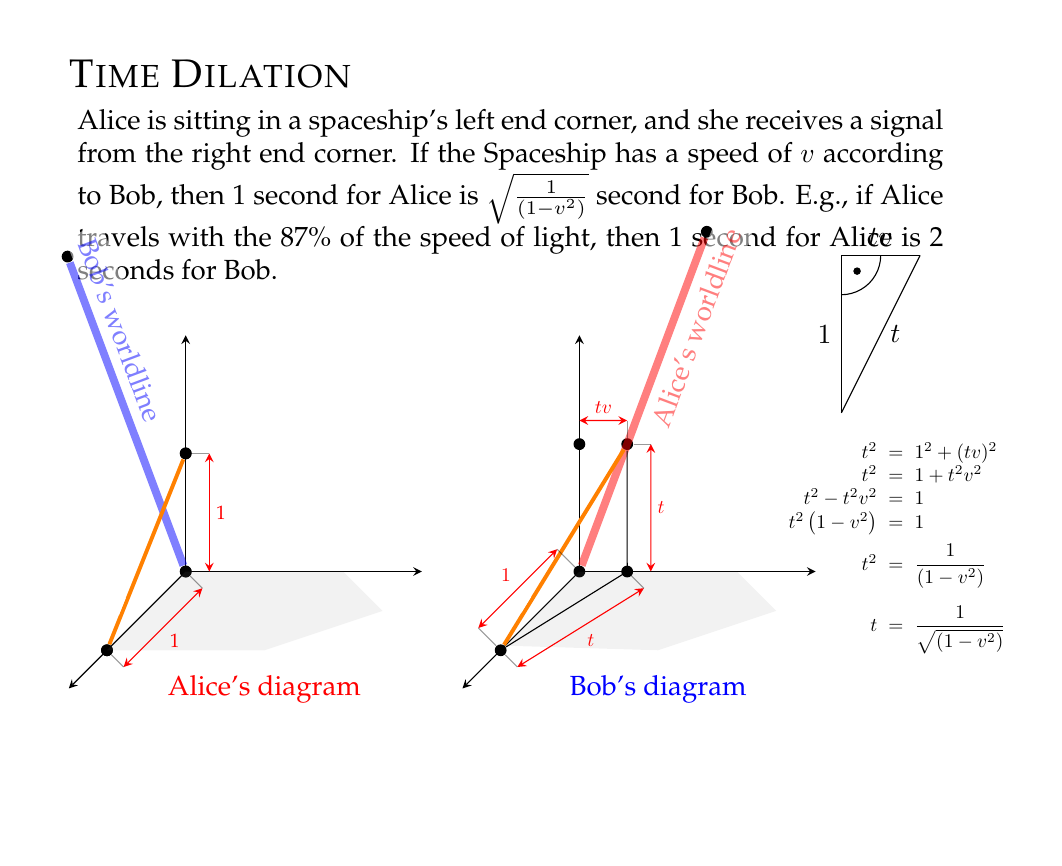
\begin{tikzpicture}[>=stealth, scale=1,
world/.style={inner sep=0, minimum size=.15cm, fill=black, circle},
worldline/.style={line width=1mm, rounded corners=1pt, opacity=.5},
axis/.style={->},
light/.style={orange, line width=.5mm},
]
\pgfmathdeclarefunction{XLorentz}{3}{\pgfmathparse{(#2 - #1*#3)/(sqrt(1-(#1)^2))}} % speed, spacecoord, timecoord
\pgfmathdeclarefunction{YLorentz}{3}{\pgfmathparse{(#3 - #1*#2)/(sqrt(1-(#1)^2))}} % speed, spacecoord, timecoord
\pgfmathsetmacro{\ThirdAxisAngle}{-135}
\pgfmathsetmacro{\ThirdAxisUnit}{.7}

%%%%%%%%%%%%%%%%%%%%%%%% DIA KEZDETE %%%%%%%%%%%%%%%%%%%%%%%%%%%

\node[anchor=north west, inner sep=0] at (0.5,8.5) {\textsc{\Large Time Dilation}}; %%%%%%% TITLE
%\node[anchor=north west, inner sep=0] at (0.5,8) {\textsc{\normalsize Role of Light}}; %%%%%%% SUBTITLE
\draw[white]  %%%%%%%%%%%% SIZE OF THE SLIDE
      (0,0) rectangle (12.77,8.9);
%%%%%%%%% TEXT %%%%%%%%%%%%%
\node[anchor=north west] at (0.5,8) {\begin{minipage}{11cm}
Alice is sitting in a spaceship's left end corner, and she receives a
signal from the right end corner. If the Spaceship has a speed of
$v$ according to Bob, then 1 second for Alice is
$\sqrt{\frac{1}{\left(1-v^2\right)}}$ second for Bob. E.g., if Alice travels with the 87\% of the speed of light, then 1 second for Alice is 2 seconds for Bob.
\end{minipage}
};
%%%%%%%%%%%%%%%%%%%%%%%% KOORDINÁTARENDSZEREK %%%%%%%%%%%%%%%%%%%%%%%%%%%
\coordinate(O1) at (2,2) {} {};
  \ThreeDimCoordSys{O1}{3}{3}{3}
\coordinate(O2) at (7,2) {} {};
  \ThreeDimCoordSys{O2}{3}{3}{3}

%%%%%%%%%%
%% SETTINGS %%
%%%%%%%%%%

\coordinate (AliceStart) at (O1);
\coordinate (AliceEnd) at (2,6) {} {} {};
\coordinate (BobStart) at (O1); % Fontos hogy átmenjen az Origón, különben rossz a lorentz transzformáció!!
\coordinate (BobEnd) at (0.5,6) {} {} {};
\coordinate (SignalStart) at (1,1) {} {} {};
\coordinate (SignalBounced) at (2,3.5) {} {} {};

%%%%%%%%%%% Ezt lehetne macronak, speedszámítócuccnak
\path (BobStart); \pgfgetlastxy{\XCoord}{\YCoord}; % Extracting coordinates of the Origin
\pgfmathsetmacro{\XFirst}{\XCoord} % Saving X coordinate
\pgfmathsetmacro{\YFirst}{\YCoord} % Saving Y coordinate
\path (BobEnd); \pgfgetlastxy{\XCoord}{\YCoord}; % Extracting coordinates of the Point
\pgfmathsetmacro{\XSecond}{\XCoord} % Saving X coordinate
\pgfmathsetmacro{\YSecond}{\YCoord} % Saving Y coordinate
\pgfmathsetmacro{\SpeedBob}{(\XFirst-\XSecond)/(\YFirst-\YSecond)} % Relativizing to the origin
%%%%%%%%%%%%%%%%%%%%%%%%%%%%%%%%%%%

\Lorentz{O1}{O1}{0}{BobStart}{BS}
\Lorentz{O1}{O1}{0}{BobEnd}{BE}
\Lorentz{O1}{O1}{0}{SignalStart}{SS}
\Lorentz{O1}{O1}{0}{SignalBounced}{SB}
\Lorentz{O1}{O1}{0}{AliceStart}{AS}
%\Lorentz{O1}{O1}{0}{AliceEnd}{AE}
\Lorentz{O1}{O1}{0}{SignalStart}{SS}
\Lorentz{O1}{O1}{0}{SignalBounced}{SB}

\Lorentz{O1}{O2}{\SpeedBob}{AliceStart}{AS'}
\Lorentz{O1}{O2}{\SpeedBob}{AliceEnd}{AE'}
\Lorentz{O1}{O2}{0}{SignalStart}{SS'}
\Lorentz{O1}{O2}{\SpeedBob}{SignalBounced}{SB'}

\node[rotate=0, text=red, fill=white] at (3,0.5) {Alice's diagram};
\node[rotate=0, text=blue, fill=white] at (8,0.5) {Bob's diagram};
\draw[worldline, blue] (BS)--(BE) node[fill=white, sloped, above, pos=.75]{Bob's worldline};
\draw[worldline, red] (AS')--(AE') node[fill=white, sloped, below, pos=.75]{Alice's worldline};
\draw[light]  (SS)-- (SB) node[fill=white, sloped, above, pos=.2]{};
\draw[light]  (SS')-- (SB') node[fill=white, sloped, above, pos=.2]{};


\coordinate(Spaceship1) at (4,2) {};
\coordinate(Spaceship2) at (4.5,1.5) {};
\coordinate(Spaceship3) at (3,1) {};
\fill[fill opacity=.1, fill=gray]  (SignalStart) -- (O1) -- (Spaceship1)
-- (Spaceship2) -- (Spaceship3)--cycle;

\coordinate(Spaceship1') at (9,2) {};
\coordinate(Spaceship2') at (9.5,1.5) {};
\coordinate(Spaceship3') at (8,1) {};
\fill[fill opacity=.1, fill=gray]  (SS') -- (O2) -- (Spaceship1')
-- (Spaceship2') -- (Spaceship3')--cycle;

\pause %%%%%% PAUSE %%%%%%%%%%%
\DistanceLabel{SS}{AS}{-45}{3 mm}{pos=.5, below right}{1}
\DistanceLabel{AS}{SB}{0}{3 mm}{pos=.5, right}{1}
\pause %%%%%% PAUSE %%%%%%%%%%%
\coordinate(r'SB') at ([yshift=-5cm]SB');
 \path[name path=Reflecting'SB'] (SB')--(r'SB');
\node[world,name intersections={of=XAxisO2 and Reflecting'SB', by=R'}] at (R'){};
\draw (R')--(SB');
\DistanceLabel{R'}{SB'}{0}{3 mm}{pos=.5, right}{$t$}
\pause %%%%%% PAUSE %%%%%%%%%%%
\draw (R')--(SS');
\DistanceLabel{R'}{SS'}{-45}{3 mm}{pos=.5, below right}{$t$}
\pause %%%%%% PAUSE %%%%%%%%%%%
 \coordinate(rSB') at ([xshift=-5cm]SB');
 \path[name path=ReflectingSB'] (SB')--(rSB');
\node[world,name intersections={of=YAxisO2 and ReflectingSB', by=R}] at (R){};
\DistanceLabel{R}{SB'}{90}{3 mm}{pos=.5, above}{$tv$}
%\DistanceLabel{O2}{R'}{90}{3 mm}{pos=.5, above, scale=.7, black}{$tv$}
\pause %%%%%% PAUSE %%%%%%%%%%%
\DistanceLabel{O2}{SS'}{135}{4 mm}{pos=.5, above left}{$1$}

\pause %%%%%% PAUSE %%%%%%%%%%%

\coordinate (v2) at (10.3264,6.0152) {} {};
\coordinate (v1) at (10.3264,4.0152) {} {};
\coordinate (v3) at (11.3264,6.0152) {} {};
\draw (v1)--(v2) node [midway, left]{$1$};
\draw (v2)--(v3) node [midway, above]{$tv$};
\draw (v3)--(v1) node [midway, right]{$t$};
\draw (10.8264,6.0152) arc (0.0009:-90.0055:0.5);
\draw[fill=black] ([xshift=  2mm, yshift= - 2mm]v2) circle (.4mm);
\node[anchor=north west, scale=.7] at (9.5,4) {\begin{minipage}{2cm}\[ \arraycolsep=1mm \begin{array}{rcl}
    t^2 &=& 1^2 + (tv)^2
\\ t^2 &=& 1 + t^2v^2
\\ t^2-t^2v^2&=&1
\\ t^2\left(1-v^2\right)&=&1
\\[1ex] t^2&=& \displaystyle  \frac{1}{\left(1-v^2\right)}
%\\[1.5em] t&=&\displaystyle \sqrt{\frac{1}{\left(1-v^2\right)}}
\\[1.5em] t&=&\displaystyle \frac{1}{\sqrt{\left(1-v^2\right)}}
\end{array}\]\end{minipage}};

\end{tikzpicture}\]
\end{frame}
\begin{frame}[fragile]
\vspace{-.55cm}
\[\hspace{-1cm}
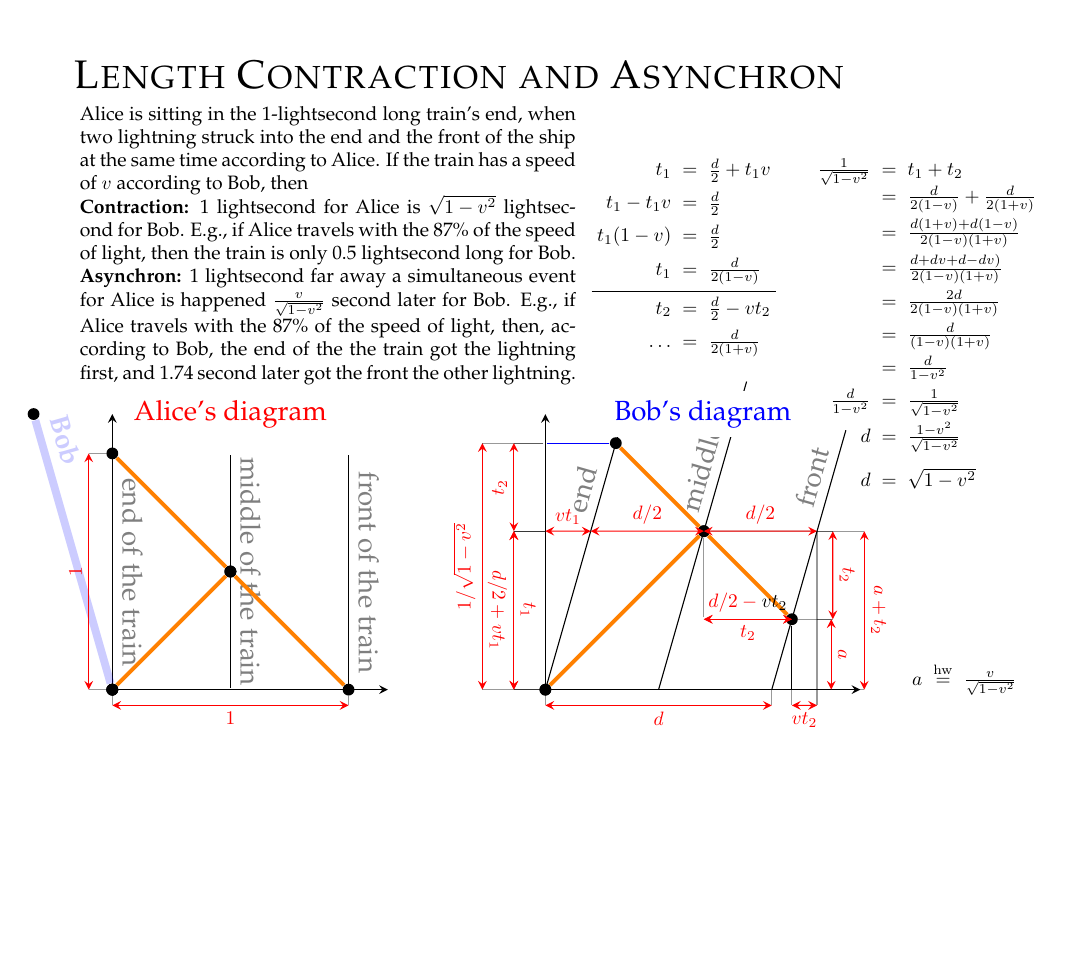
\begin{tikzpicture}[>=stealth, scale=1,
world/.style={inner sep=0, minimum size=.15cm, fill=black, circle},
worldline/.style={line width=1mm, rounded corners=1pt, opacity=.5},
axis/.style={->},
light/.style={orange, line width=.5mm},
]
\pgfmathdeclarefunction{XLorentz}{3}{\pgfmathparse{(#2 - #1*#3)/(sqrt(1-(#1)^2))}} % speed, spacecoord, timecoord
\pgfmathdeclarefunction{YLorentz}{3}{\pgfmathparse{(#3 - #1*#2)/(sqrt(1-(#1)^2))}} % speed, spacecoord, timecoord
\pgfmathsetmacro{\ThirdAxisAngle}{-135}
\pgfmathsetmacro{\ThirdAxisUnit}{.7}

%%%%%%%%%%%%%%%%%%%%%%%% DIA KEZDETE %%%%%%%%%%%%%%%%%%%%%%%%%%%

\node[anchor=north west, inner sep=0] at (0.5,8.5) {\textsc{\Large Length Contraction and Asynchron}}; %%%%%%% TITLE
%\node[anchor=north west, inner sep=0] at (0.5,8) {\textsc{\normalsize Role of Light}}; %%%%%%% SUBTITLE
\draw[white]  %%%%%%%%%%%% SIZE OF THE SLIDE
      (0,0) rectangle (12.77,8.9);
%%%%%%%%% TEXT %%%%%%%%%%%%%
\node[anchor=north west, fill=white, fill opacity=1, text opacity=1,scale=.7] at (0.5,8)
{\begin{minipage}{9cm}
Alice is sitting in the 1-lightsecond long train's end, when two lightning struck into
the end and the front of the ship at the same time according to Alice.  If the train has a speed of $v$ according to Bob, then
\\ \textbf{Contraction:} 1 lightsecond for Alice is
$\sqrt{1-v^2}$ lightsecond for Bob.
E.g., if Alice travels with the 87\%
of the speed of light, then the train is only 0.5 lightsecond long for Bob.
\\ \textbf{Asynchron:} 1 lightsecond far away a simultaneous event for Alice is happened
$\frac v{\sqrt{1-v^2}}$ second later for Bob.
E.g., if Alice travels with the 87\%
of the speed of light, then, according to Bob, the end of the the train got the lightning first, and 1.74 second later got the front the other lightning.
\end{minipage}
};
%%%%%%%%%%%%%%%%%%%%%%%% KOORDINÁTARENDSZEREK %%%%%%%%%%%%%%%%%%%%%%%%%%%
\coordinate(O1) at (1,0.5) {} {} {} {} {} {};
  \OneQuadrantCoordSys{O1}{3.5}{3.5}{3}
\coordinate(O2) at (6.5,0.5) {} {} {} {} {} {} {} {} {} {};
  \OneQuadrantCoordSys{O2}{4}{3.5}{3}

%%%%%%%%%%
%% SETTINGS %%
%%%%%%%%%%

\coordinate (AliceStart) at (O1);
\coordinate (AliceEnd) at (1,4) {} {} {} {} {} {} {} {};
\coordinate (BobStart) at (O1); % Fontos hogy átmenjen az Origón, különben rossz a lorentz transzformáció!!
\coordinate (BobEnd) at (0,4) {} {} {} {} {} {} {} {} {} {} {};
\coordinate (SignalStart) at (O1) {} {} {} {} {};
\coordinate (SignalStart2) at (4,0.5) {} {} {} {} {} {} {} {} {} {} {};
\coordinate (SignalBounced) at (2.5,2) {} {} {} {} {} {} {} {} {} {} {};
\coordinate (SignalEnd) at (1,3.5) {};

%%%%%%%%%%% Ezt lehetne macronak, speedszámítócuccnak
\path (BobStart); \pgfgetlastxy{\XCoord}{\YCoord}; % Extracting coordinates of the Origin
\pgfmathsetmacro{\XFirst}{\XCoord} % Saving X coordinate
\pgfmathsetmacro{\YFirst}{\YCoord} % Saving Y coordinate
\path (BobEnd); \pgfgetlastxy{\XCoord}{\YCoord}; % Extracting coordinates of the Point
\pgfmathsetmacro{\XSecond}{\XCoord} % Saving X coordinate
\pgfmathsetmacro{\YSecond}{\YCoord} % Saving Y coordinate
\pgfmathsetmacro{\SpeedBob}{(\XFirst-\XSecond)/(\YFirst-\YSecond)} % Relativizing to the origin
%%%%%%%%%%%%%%%%%%%%%%%%%%%%%%%%%%%

\Lorentz{O1}{O1}{0}{BobStart}{BS}
\Lorentz{O1}{O1}{0}{BobEnd}{BE}
\Lorentz{O1}{O1}{0}{SignalStart}{SS}
\Lorentz{O1}{O1}{0}{SignalStart2}{SS2}
\Lorentz{O1}{O1}{0}{SignalBounced}{SB}
\Lorentz{O1}{O1}{0}{AliceStart}{AS}
%\Lorentz{O1}{O1}{0}{AliceEnd}{AE}
\Lorentz{O1}{O1}{0}{SignalStart}{SS}
\Lorentz{O1}{O1}{0}{SignalBounced}{SB}
\Lorentz{O1}{O1}{0}{SignalEnd}{SE}

\Lorentz{O1}{O2}{\SpeedBob}{AliceStart}{AS'}
%\Lorentz{O1}{O2}{\SpeedBob}{AliceEnd}{AE'}
\Lorentz{O1}{O2}{\SpeedBob}{SignalStart}{SS'}
\Lorentz{O1}{O2}{\SpeedBob}{SignalStart2}{SS2'}
\Lorentz{O1}{O2}{\SpeedBob}{SignalBounced}{SB'}
\Lorentz{O1}{O2}{\SpeedBob}{SignalEnd}{SE'}


\node[inner sep=0] (v4) at (2.5,0.5) {};
\node[inner sep=0] (v5) at (2.5,3.5) {};
\node[inner sep=0] (v6) at (4,3.5) {};
\node[inner sep=0] (v7) at ([yshift=3 cm]O1) {};

\draw  (v5) -- (v4) node[opacity=.5, midway, sloped, above]{middle of the train};
\draw  (v6) -- (SignalStart2)node[opacity=.5, midway, sloped, above]{front of the train};
\draw  (v7) -- (O1)node[opacity=.5, midway, sloped, above]{end of the train};


\pgfmathsetmacro{\y}{3.75}
\pgfmathsetmacro{\x}{-\y*\SpeedBob}
\coordinate (TrainBackEnd) at ([yshift=\y cm,xshift=\x cm]O2){};
\pgfmathsetmacro{\y}{-3}
\pgfmathsetmacro{\x}{-\y*\SpeedBob}
\coordinate (TrainFrontStartRef) at ([yshift= \y cm , xshift= \x cm ]SS2');
\pgfmathsetmacro{\y}{2.4}
\pgfmathsetmacro{\x}{-\y*\SpeedBob}
\coordinate (TrainFrontEnd) at ([yshift= \y cm , xshift= \x cm ]SS2');
\pgfmathsetmacro{\y}{1.9}
\pgfmathsetmacro{\x}{-\y*\SpeedBob}
\coordinate (TrainMiddleEnd) at ([yshift= \y cm , xshift= \x cm ]SB');
\pgfmathsetmacro{\y}{-4}
\pgfmathsetmacro{\x}{-\y*\SpeedBob}
\coordinate (TrainMiddleStartRef) at ([yshift= \y cm , xshift= \x cm ]SB');

\draw[name path=EndLine] (O2)--(TrainBackEnd) node [above, pos=.66, sloped, opacity=.5]{end};
\path[name path=KisebbFrontLine] (SS2')--(TrainFrontStartRef);
\path[name intersections={of=XAxisO2 and KisebbFrontLine, by=R}](R);
\coordinate(TrainFrontStart) at (R);
\draw[name path=FrontLine] (TrainFrontEnd)--(TrainFrontStart) node [above, pos=.2, sloped, opacity=.5]{front};

\path[name path=MiddleLine] (SB')--(TrainMiddleStartRef);
\path[name intersections={of=XAxisO2 and MiddleLine, by=R'}](R'){};
\coordinate(TrainMiddleStart) at (R');
\draw (TrainMiddleStart)--(TrainMiddleEnd) node [above, pos=.7, sloped, opacity=.5]{middle};

\coordinate(VetSB') at ([xshift=-5cm]SB');
\coordinate(VisszaVetSB') at ([xshift=4cm]SB');
\path[name path=MiddleHorizontal] (VisszaVetSB')--(VetSB');
\node[name intersections={of=EndLine and MiddleHorizontal, by=D}](Dnode) at (D){};
\node[name intersections={of=FrontLine and MiddleHorizontal, by=C}](Cnode) at (C){};
\coordinate(CRef) at ([yshift=-5cm]C);
\path[name path=UtolsoVertical] (C)--(CRef);
\path[name intersections={of=UtolsoVertical and XAxisO2, by=Talp}](Talp){};

\coordinate(MiddleVerticalRef) at ([yshift=-4cm]SB');
\path[name path=MiddleVertical] (MiddleVerticalRef)--(SB');

\coordinate(VetSS2') at ([xshift=-5cm]SS2');
\coordinate(VisszaVetSS2') at ([xshift=2cm]SS2');
\path[name path=FrontHorizontal] (VisszaVetSS2')--(VetSS2');
\path[name intersections={of=FrontHorizontal and UtolsoVertical, by=t1t2}] (t1t2){};

\node[rotate=0, text=red, fill=white] at (2.5,4) {Alice's diagram};
\node[rotate=0, text=blue, fill=white] at (8.5,4) {Bob's diagram};
\draw[worldline, blue, opacity=.2] (BS)--(BE) node[opacity=.2, sloped, above, pos=.9]{\textbf{Bob}};
%\draw[worldline, red] (AS')--(AE') node[fill=white, sloped, above, pos=.75]{Alice};
\draw[light]  (SS)-- (SB);
\draw[light]  (SB)-- (SE);
\draw[light]  (SS')-- (SB');
\draw[light]  (SS2)-- (SB);
\draw[light]  (SS2')-- (SB');
\draw[light]  (SB')-- (SE');

\node[world] at (SB){};
\node[world] at (SB'){};

\path(SB')|- node[inner sep=0](kozepe){}(SS2');

\pause %%%%%% PAUSE %%%%%%%%%%%
\DistanceLabel{O1}{SE}{180}{3 mm}{pos=.5, above, sloped}{$1$}
\pause %%%%%% PAUSE %%%%%%%%%%%
\DistanceLabel{SS2}{O1}{-90}{2 mm}{pos=.5, below, sloped}{$1$}
\pause %%%%%% PAUSE %%%%%%%%%%%
\DistanceLabel{R}{O2}{-90}{2 mm}{pos=.5, below}{$d$}
\pause %%%%%% PAUSE %%%%%%%%%%%
%%%%%%%%%%%%%%%%%%
\coordinate(Vet2SS2') at ([yshift=-3cm]SS2');
\path[name path=FrontVertical] (SS2')--(Vet2SS2');
\draw[name intersections={of=FrontVertical and XAxisO2, by=VF}] (SS2') -- (VF);
\DistanceLabel{SS2'}{VF}{0}{5 mm}{pos=.5, rotate=-90, above}{$a$}
\pause %%%%%% PAUSE %%%%%%%%%%%
\path[world, name intersections={of=YAxisO2 and MiddleHorizontal, by=A}](A){};
%\node[world](Anode) at (A){};
\path(SE')-| node[inner sep=0](SE'N){}(A);
\draw[blue] (SE')--(SE'N);
\DistanceLabel{O2}{SE'N}{180}{8 mm}{pos=.5, above, sloped}{$1/\sqrt{1-v^2}$}
\pause %%%%%% PAUSE %%%%%%%%%%%
%\draw[blue] (A)--(C);
\DistanceLabel{D}{SB'}{90}{0 mm}{pos=.5, above}{$d/2$}
\pause %%%%%% PAUSE %%%%%%%%%%%
\DistanceLabel{A}{O2}{180}{4 mm}{pos=.5, sloped, above}{$t_1$}
\pause %%%%%% PAUSE %%%%%%%%%%%
\DistanceLabel{A}{D}{90}{0 mm}{pos=.5, above}{$vt_1$}
\pause %%%%%% PAUSE %%%%%%%%%%%
\DistanceLabel{A}{O2}{180}{4 mm}{pos=.5, below, sloped}{$d/2+vt_1$}
\pause %%%%%% PAUSE %%%%%%%%%%%
\DistanceLabel{SE'N}{A}{180}{4 mm}{pos=.5, rotate=90, above}{$t_2$}
\pause %%%%%% PAUSE %%%%%%%%%%%
\draw[opacity=.4] (SB')--(C);
\DistanceLabel{t1t2}{C}{0}{2 mm}{pos=.5, rotate=-90, above}{$t_2$}
\pause %%%%%% PAUSE %%%%%%%%%%%
\DistanceLabel{C}{Talp}{0}{6 mm}{pos=.5, above, sloped}{$a+t_2$}
\pause %%%%%% PAUSE %%%%%%%%%%%
\DistanceLabel{SB'}{C}{90}{0 mm}{pos=.5, above}{$d/2$}
\pause %%%%%% PAUSE %%%%%%%%%%%
\draw[opacity=.4] (C)--(Talp);
\DistanceLabel{VF}{Talp}{-90}{2 mm}{pos=.5, below}{$vt_2$}
\pause %%%%%% PAUSE %%%%%%%%%%%
\draw[opacity=.4] (kozepe)--(SB');
\DistanceLabel{kozepe}{SS2'}{0}{0 mm}{pos=.5, above}{$d/2-\textcolor{black}{vt_2}$}
\pause %%%%%% PAUSE %%%%%%%%%%%
\DistanceLabel{kozepe}{SS2'}{0}{0 mm}{pos=.5, below}{$t_2$}

\pause %%%%%% PAUSE %%%%%%%%%%%


\node[anchor=north west, scale=.7] at (7,7.6) {\begin{minipage}{2cm}\[ \arraycolsep=1mm \begin{array}{rcl}
    t_1 &=& \frac d2+t_1v
\\[1ex] t_1-t_1v &=& \frac d2
\\[1ex] t_1(1-v) &=& \frac d2
\\[1ex] t_1 &=& \frac d{2(1-v)}
%\end{array}
%\;
%\begin{array}{rcl}
\\[1ex] \hline
\\[-2ex]t_2&=& \frac d2-vt_2
%\\[1ex] t_2+vt_2&=& \frac d2
%\\[1ex] t_2(1+v)&=& \frac d2
\\[1ex]% t_2
\dots &=& \frac d{2(1+v)}
\end{array}\]
\end{minipage}};

\node[anchor=north west, scale=.7] at (9.8,7.6) {
\begin{minipage}{2cm}
\[ \arraycolsep=1mm \begin{array}{rcl}
                    \frac{1}{\sqrt{1-v^2}}  &=&t_1+t_2
\\         &=&\frac d{2(1-v)}+\frac d{2(1+v)}
\\[1ex] &=&\frac {d(1+v)+d(1-v)}{2(1-v)(1+v)}
\\[1ex] &=&\frac {d+dv+d-dv)}{2(1-v)(1+v)}
\\[1ex] &=&\frac {2d}{2(1-v)(1+v)}
\\[1ex] &=&\frac {d}{(1-v)(1+v)}
\\[1ex] &=&\frac {d}{1-v^2}
%\end{array}\]
%\end{minipage}};
%
%\node[anchor=north west, scale=.7] at (10,5.8) {
%\begin{minipage}{2cm}
%\[ \arraycolsep=1mm \begin{array}{rcl}
%\\[1ex] \hline
%\\[-2ex]
\\[1ex] \frac {d}{1-v^2} &=&\frac{1}{\sqrt{1-v^2}}
\\[1ex] d&=&\frac{1-v^2}{\sqrt{1-v^2}}
\\[1em] d&=&\sqrt{1-v^2}
%\end{array}\]
%\end{minipage}};
%
%\node[anchor=north west, scale=.7] at (10.2,4.2) {
%\begin{minipage}{2cm}
%\[ \arraycolsep=1mm \begin{array}{rcl}
%\\[1ex] \hline
%\\[5ex]
%a  %&=&t_1-t_2
%\\ &=&\frac d{2(1-v)}-\frac d{2(1+v)}
%\\[1ex] &=&\frac {d(1+v)-d(1-v)}{2(1-v)(1+v)}
%\\[1ex] &=&\frac {d+dv-d+dv)}{2(1-v)(1+v)}
%\\[1ex] &=&\frac {2dv}{2(1-v)(1+v)}
%\\[1ex] &=&\frac {dv}{1-v^2}
%\\[1ex] &=& \frac {v\sqrt{1-v^2} }{1-v^2}
%\\[1ex]
%&\overset{\mathrm{hw}}{=}& \frac {v }{\sqrt{1-v^2}}
\end{array}\]
\end{minipage}};

\node[anchor=north west, scale=.7] at (11,1.2) {
\begin{minipage}{2cm}
\[ \arraycolsep=1mm \begin{array}{rcl}
%\\[1ex] \hline
%\\[5ex]
a  %&=&t_1-t_2
&\overset{\mathrm{hw}}{=}& \frac {v }{\sqrt{1-v^2}}
\end{array}\]
\end{minipage}};

\end{tikzpicture}\]
\end{frame}

%%%%%%%%%%%%%%%%%%%%%%%%%% SLIDE %%%%%%%%%%%%%%%%%%%%%%%%%%

\szakasz[Lorentz Transformation]{Lorentz Transformation}

\begin{frame}[fragile]
\vspace{-.55cm}
\[\hspace{-1cm}
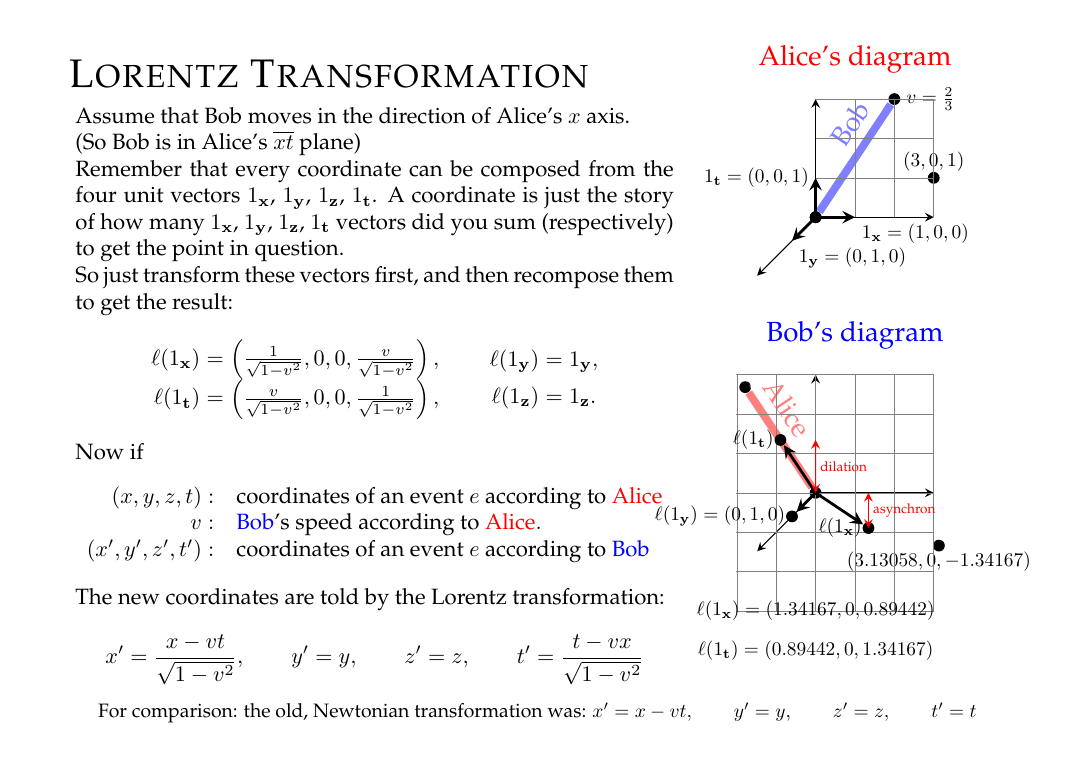
\begin{tikzpicture}[>=stealth, scale=1,
world/.style={inner sep=0, minimum size=.15cm, fill=black, circle},
worldline/.style={line width=1mm, rounded corners=1pt, opacity=.5},
axis/.style={->},
light/.style={orange, line width=.5mm},
]
\pgfmathdeclarefunction{XLorentz}{3}{\pgfmathparse{(#2 - #1*#3)/(sqrt(1-(#1)^2))}} % speed, spacecoord, timecoord
\pgfmathdeclarefunction{YLorentz}{3}{\pgfmathparse{(#3 - #1*#2)/(sqrt(1-(#1)^2))}} % speed, spacecoord, timecoord
\pgfmathsetmacro{\ThirdAxisAngle}{-135}
\pgfmathsetmacro{\ThirdAxisUnit}{.7}

%%%%%%%%%%%%%%%%%%%%%%%% DIA KEZDETE %%%%%%%%%%%%%%%%%%%%%%%%%%%

\node[anchor=north west, inner sep=0] at (0.5,8.5) {\textsc{\Large Lorentz Transformation}}; %%%%%%% TITLE
%\node[anchor=north west, inner sep=0] at (0.5,8) {\textsc{\normalsize Role of Light}}; %%%%%%% SUBTITLE
\draw[white]  %%%%%%%%%%%% SIZE OF THE SLIDE
      (0,0) rectangle (12.77,8.9);
%%%%%%%%% TEXT %%%%%%%%%%%%%
\node[anchor=north west, scale=.8] at (0.5,8) {\begin{minipage}{9.5cm}
Assume that Bob moves in the direction of Alice's $x$ axis.
\\ (So Bob is in Alice's $\overline{xt}$ plane)

Remember that every coordinate can be composed from the four unit vectors
$1_{\mathbf x}$, $1_{\mathbf y}$, $1_{\mathbf z}$, $1_{\mathbf t}$.
 {A coordinate is just the story of how many $1_{\mathbf x}$, $1_{\mathbf y}$, $1_{\mathbf z}$, $1_{\mathbf t}$ vectors did you sum (respectively) to get the point in question.}

So just transform these vectors first, and then recompose them to get the result:
\[\arraycolsep=.5mm\begin{array}{rcl}
\ell (1_{\mathbf x}) &=& \left( \frac 1{\sqrt{1-v^2}}, 0,0,\frac v{\sqrt{1-v^2}}\right),
\\ \ell (1_{\mathbf t}) &=& \left( \frac v{\sqrt{1-v^2}}, 0,0,\frac 1{\sqrt{1-v^2}}\right),
\end{array}\qquad
\begin{array}{rcl}
 \ell (1_{\mathbf y}) &=& 1_{\mathbf y},
\\[1ex] \ell (1_{\mathbf z}) &=& 1_{\mathbf z}.
\end{array}
\]
Now if
\[\begin{array}{rl}
(x,y,z,t) : & \textup{coordinates of an event $e$ according to \textcolor{red}{Alice}}
\\ v: & \textup{\textcolor{blue}{Bob}'s speed according to \textcolor{red}{Alice}}.
\\ (x',y',z',t'): & \textup{coordinates of an event $e$ according to \textcolor{blue}{Bob}}
\end{array}
\]
The new coordinates are told by the Lorentz transformation:
%\[\begin{array}{rcl}
%    x'&=&\frac{x-vt}{\sqrt{1-v^2}}
%\\ y'&=& y
%\\ z'&=& z
%\\ t'&=&\frac{t-vx}{\sqrt{1-v^2}}
%\end{array}\]
\[x'=\frac{x-vt}{\sqrt{1-v^2}}, \qquad y'=y, \qquad z'=z,\qquad t'=\frac{t-vx}{\sqrt{1-v^2}}\]
\end{minipage}
};
%%%%%%%%%%%%%%%%%%%%%%%% KOORDINÁTARENDSZEREK %%%%%%%%%%%%%%%%%%%%%%%%%%%
\coordinate(O1) at (10,6.5) {} {} {} {} {} {} {};
  \ThreeDimCoordSys{O1}{1.5}{1.5}{1.5}
\coordinate(O2) at (10,3) {} {} {} {} {} {} {} {};
  \ThreeDimCoordSys{O2}{1.5}{1.5}{1.5}

%%%%%%%%%%
%% SETTINGS %%
%%%%%%%%%%

\coordinate (AliceStart) at (O1);
\coordinate (AliceEnd) at (10,7.5) {} {} {} {} {} {} {} {} {} {} {};
\coordinate (BobStart) at (O1); % Fontos hogy átmenjen az Origón, különben rossz a lorentz transzformáció!!
\coordinate (BobEnd) at (11,8) {} {} {} {} {} {} {} {} {} {} {} {} {};

%%%%%%%%%%% Ezt lehetne macronak, speedszámítócuccnak
\path (BobStart); \pgfgetlastxy{\XCoord}{\YCoord}; % Extracting coordinates of the Origin
\pgfmathsetmacro{\XFirst}{\XCoord} % Saving X coordinate
\pgfmathsetmacro{\YFirst}{\YCoord} % Saving Y coordinate
\path (BobEnd); \pgfgetlastxy{\XCoord}{\YCoord}; % Extracting coordinates of the Point
\pgfmathsetmacro{\XSecond}{\XCoord} % Saving X coordinate
\pgfmathsetmacro{\YSecond}{\YCoord} % Saving Y coordinate
\pgfmathsetmacro{\SpeedBob}{(\XFirst-\XSecond)/(\YFirst-\YSecond)} % Relativizing to the origin
%%%%%%%%%%%%%%%%%%%%%%%%%%%%%%%%%%%

\Lorentz{O1}{O1}{0}{BobStart}{BS}
\Lorentz{O1}{O1}{0}{BobEnd}{BE}
\Lorentz{O1}{O1}{0}{AliceStart}{AS}
%\Lorentz{O1}{O1}{0}{AliceEnd}{AE}
\Lorentz{O1}{O2}{\SpeedBob}{AliceStart}{AS'}
\Lorentz{O1}{O2}{\SpeedBob}{AliceEnd}{AE'}
\node[world] (e) at (11.5,7) {};
%\node[anchor=south] at (e) {$(x,y,z,t)$};
\node[anchor=south, scale=.7] at (e) {$(3,0,1)$};
\node[anchor=west, scale=.7, inner sep=6] at (BobEnd) {$v=\frac 23$};
\Lorentz{O1}{O2}{\SpeedBob}{e}{e'}
%\node[anchor=north] at (e') {$\left(\frac{x-vt}{\sqrt{1-v^2}}, y, z, \frac{t-vx}{\sqrt{1-v^2}}\right)$};

\pgfmathsetmacro{\X}{(3 - 1*2/3)/(sqrt(1-(2/3)^2))}
\pgfmathsetmacro{\T}{(1 - 3*2/3)/(sqrt(1-(2/3)^2))}
\node[anchor=north, scale=.7] at (e') {$\left( \X, 0, \T\right)$};

\node[rotate=0, text=red, fill=white] at (10.5,8.5) {Alice's diagram};
\node[rotate=0, text=blue, fill=white] at (10.5,5) {Bob's diagram};
\draw[worldline, blue] (BS)--(BE) node[fill=white, sloped, above, pos=.7]{Bob};
\draw[worldline, red] (AS')--(AE') node[fill=white, sloped, above, pos=.7]{Alice};

%\node[scale=.7] at (10,1) {\begin{minipage}{5cm}The illustration is faithful for
%
%\vspace{-1em}
%\[(x,y,z,t)= (3,0,0,1)\]\end{minipage}};
\coordinate (v1) at (10,7) {};
\coordinate (v2) at (10.5,6.5) {};
\coordinate (v3) at (9.70,6.20) {};
\begin{scope}[line width=1]
\draw[->]  (O1) -- (v1);
\draw[->]  (O1) -- (v2);
\draw[->]  (O1) -- (v3);
\end{scope}
\node[scale=.7, anchor=east] at (v1){$1_{\mathbf t} = (0,0,1)$};
\node[scale=.7, anchor=north west] at (v2){$1_{\mathbf x} = (1,0,0)$};
\node[scale=.7, anchor=north west] at (v3){$1_{\mathbf y} = (0,1,0)$};
\draw [help lines, step=.5cm] (O1) grid (XYO1);
\draw [help lines, step=.5cm] ([yshift=-1.501cm, xshift=-1.01cm]O2) grid (XYO2);
\Lorentz{O1}{O2}{\SpeedBob}{v1}{v1'}
\Lorentz{O1}{O2}{\SpeedBob}{v2}{v2'}
\Lorentz{O1}{O2}{0}{v3}{v3'}
\begin{scope}[line width=1]
\draw[->]  (O2) -- (v1');
\draw[->]  (O2) -- (v2');
\draw[->]  (O2) -- (v3');
\end{scope}
\pgfmathsetmacro{\X}{1/(sqrt(1-(2/3)^2))}
\pgfmathsetmacro{\T}{(2/3)/(sqrt(1-(2/3)^2))}
\node[scale=.7, anchor=east] at (v1') {$\ell(1_{\mathbf t})$};
\node[scale=.7, anchor=east] at (v2') {$\ell(1_{\mathbf x})$};
\node[scale=.7] at (10,1) {$\ell(1_{\mathbf t}) = (\T,0,\X)$};
\node[scale=.7] at (10,1.5) {$\ell(1_{\mathbf x}) = (\X,0,\T)$};
\node[scale=.7, anchor=east] at (v3'){$\ell(1_{\mathbf y}) = (0,1,0)$};
\coordinate(refx) at ([yshift=1cm]v2');
\coordinate(reft) at ([xshift=1cm]v1');
\path[name path=myvertical] (v2')--(refx);
\path[name path=myhorizontal] (v1')--(reft);
\node[inner sep=0,name intersections={of=myvertical and XAxisO2, by=vetx}] at (vetx){};
\node[inner sep=0,name intersections={of=myhorizontal and YAxisO2, by=vett}] at (vett){};
\DistanceLabel{v2'}{vetx}{0}{0 mm}{pos=.5, right, scale=.7}{asynchron}
\DistanceLabel{O2}{vett}{0}{0 mm}{pos=.5, right, scale=.7}{dilation}
\node[scale=.7, anchor=west] at (0.8,0.2) {For comparison: the old, Newtonian transformation was:
%\[\begin{array}{rcl}
%    x'&=& x-vt
%\\ y'&=& y
%\\ z'&=& z
%\\ t'&=& t
%\end{array}\]
$x'=x-vt, \qquad y'=y, \qquad z'=z,\qquad t'=t$
};
\end{tikzpicture}\]
\end{frame}

\szakasz[NoFTL]{NoFTL}


%%%%%%%%%%%%%%%%%%%%%%%%%%%%%% SLIDE %%%%%%%%%%%%%%%%%%%%%%%%%%%%%%%%%%%%%%%%%%%%%
\begin{frame}[fragile]
\vspace{-.55cm}
\[\hspace{-1cm}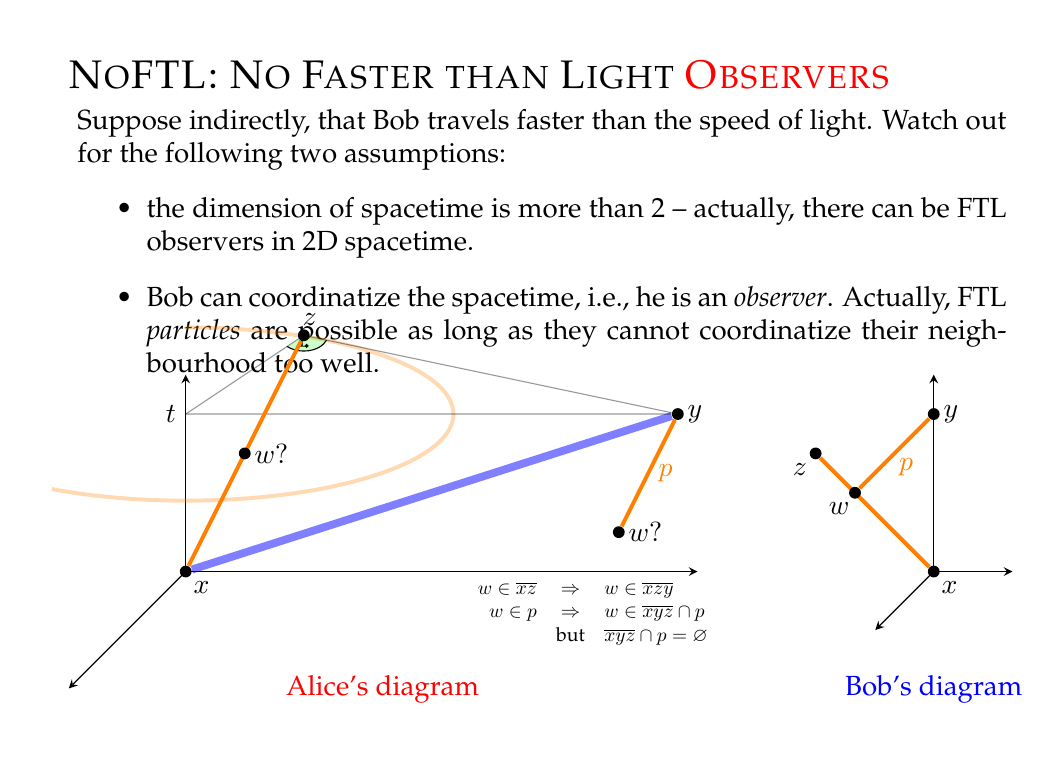
\begin{tikzpicture}[>=stealth, scale=1,
world/.style={inner sep=0, minimum size=.15cm, fill=black, circle},
worldline/.style={line width=1mm, rounded corners=1pt, opacity=.5},
axis/.style={->},
light/.style={orange, line width=.5mm},
]
\pgfmathdeclarefunction{XLorentz}{3}{\pgfmathparse{(#2 - #1*#3)/(sqrt(1-(#1)^2))}} % speed, spacecoord, timecoord
\pgfmathdeclarefunction{YLorentz}{3}{\pgfmathparse{(#3 - #1*#2)/(sqrt(1-(#1)^2))}} % speed, spacecoord, timecoord
\pgfmathsetmacro{\ThirdAxisAngle}{-135}
\pgfmathsetmacro{\ThirdAxisUnit}{.7}

%%%%%%%%%%%%%%%%%%%%%%%% DIA KEZDETE %%%%%%%%%%%%%%%%%%%%%%%%%%%

\node[anchor=north west, inner sep=0] at (0.5,8.5) {\textsc{\Large NoFTL: No Faster than Light \textcolor{red}{Observers}}}; %%%%%%% TITLE
%\node[anchor=north west, inner sep=0] at (0.5,8) {\textsc{\normalsize Role of Light}}; %%%%%%% SUBTITLE
\coordinate(jobbfelsosarok) at (12.77,8.9);
\draw[white]  %%%%%%%%%%%% SIZE OF THE SLIDE
      (0,0) rectangle (jobbfelsosarok);
%%%%%%%%% TEXT %%%%%%%%%%%%%
\node[anchor=north west, scale=1] at (0.5,8) {\begin{minipage}{11.8cm}
Suppose indirectly, that Bob travels faster than the speed of light. Watch out for the following two assumptions:
\begin{itemize}
\item the dimension of spacetime is more than 2 -- actually, there can be FTL observers in 2D spacetime.
\item Bob can coordinatize the spacetime, i.e., he is an \emph{observer}. Actually, FTL \emph{particles} %(and as such, as we will see it later, time travel)
    are possible as long as they cannot coordinatize their neighbourhood too well.
\end{itemize}
\end{minipage}
};
%%%%%%%%%%%%%%%%%%%%%%%% KOORDINÁTARENDSZEREK %%%%%%%%%%%%%%%%%%%%%%%%%%%
\coordinate(O1) at (2,2) {} {} {} {};
  \ThreeDimCoordSys{O1}{6.5}{2.5}{3}
\coordinate(O2) at (11.5,2) {} {} {} {} {};
  \ThreeDimCoordSys{O2}{1}{2.5}{1.5}

%%%%%%%%%%
%% SETTINGS %%
%%%%%%%%%%
\coordinate (BobStart) at (O1); % Fontos hogy átmenjen az Origón, különben rossz a lorentz transzformáció!!
\coordinate (BobEnd) at (1.25,6) {} {} {} {} {} {};

%%%%%%%%%%% Ezt lehetne macronak, speedszámítócuccnak
\path (BobStart); \pgfgetlastxy{\XCoord}{\YCoord}; % Extracting coordinates of the Origin
\pgfmathsetmacro{\XFirst}{\XCoord} % Saving X coordinate
\pgfmathsetmacro{\YFirst}{\YCoord} % Saving Y coordinate
\path (BobEnd); \pgfgetlastxy{\XCoord}{\YCoord}; % Extracting coordinates of the Point
\pgfmathsetmacro{\XSecond}{\XCoord} % Saving X coordinate
\pgfmathsetmacro{\YSecond}{\YCoord} % Saving Y coordinate
\pgfmathsetmacro{\SpeedBob}{(\XFirst-\XSecond)/(\YFirst-\YSecond)} % Relativizing to the origin
%%%%%%%%%%%%%%%%%%%%%%%%%%%%%%%%%%%

%\Lorentz{O1}{O1}{0}{BobStart}{BS}
%\Lorentz{O1}{O1}{0}{BobEnd}{BE}


\node[rotate=0, text=red, fill=white] at (4.5,0.5) {Alice's diagram};
\node[rotate=0, text=blue, fill=white] at (11.5,0.5) {Bob's diagram};


\node[world](x)at (O1) {};
\node[anchor=135] at (x) {$x$};
\node[world] (y) at (8.25,4) {};
\node[anchor=180] at (y) {$y$};
\draw[worldline, blue](x)--(y);

\node[world](x') at (O2){};
\node[anchor=135] at (x'){$x$};
\node[world] (y') at (11.5,4) {};
\node[anchor=180] at (y'){$y$};

\pause

\draw[light, opacity=.3] (2,5.1) arc (90:-120:3.4 and 1.1);
\coordinate(t) at ([yshift=2cm]O1);
\node[anchor=0] at (t){$t$};
\draw[opacity=.4] (y)--(t);

\pause

\coordinate(z) at at (3.5,5);

\draw[opacity=.4] (t)--(z)--(y);

\begin{scope}[shift={(0,0)}]
\clip (z)--(y)--(t)--(z);
\draw[fill=green, fill opacity=0.2, draw=black]  (z) ellipse (0.3 and 0.2);
\draw[fill=black] (3.5356,4.8666) circle (.5pt);
\end{scope}

\pause

\node[world](znode) at (z) {};
\node[anchor=250] at (z){$z$};
\draw[light] (x)--(znode);

\pause

\node[world] (z') at (10,3.5) {};
\node[anchor=45] at (z'){$z$};
\draw[light](x')--(z');

\pause

\node[world] (w') at (10.5,3) {};
\node[anchor=45] at (w'){$w$};
\draw[light](w')--(y') node[midway, below right, inner sep=1]{$p$};

\pause

\node[world] (w1) at (2.75,3.5) {};
\node[anchor=180] at (w1){$w?$};

\pause

\node[world] (w2) at ([yshift=-1.5cm, xshift=-.75 cm]y) {};
\draw[light](w2)--(y)node[midway, right, inner sep=3]{$p$};
\node[anchor=180] at (w2){$w?$};

\node[anchor=north west, scale=.7] at (5.5,2) {$\begin{array}{rcl}
\pause         w\in \overline{xz} & \Rightarrow & w \in \overline{xzy}
\pause      \\ w\in p             & \Rightarrow & w \in \overline{xyz}  \cap  p
\pause      \\                    & \textup{but}&       \overline{xyz}  \cap  p = \varnothing
     \end{array}$};
\end{tikzpicture}\]
\end{frame}

%%%%%%%%%%%%%%%%%%%%%%%%%%%%%%%%%%%%%%%%%% SLIDE %%%%%%%%%%%%%%%%%%%%%%%%%%%%%%%%%%%%%%%%%%%%%%%%%5
\begin{frame}[fragile]
\vspace{-.55cm}
\[
\hspace{-1cm}
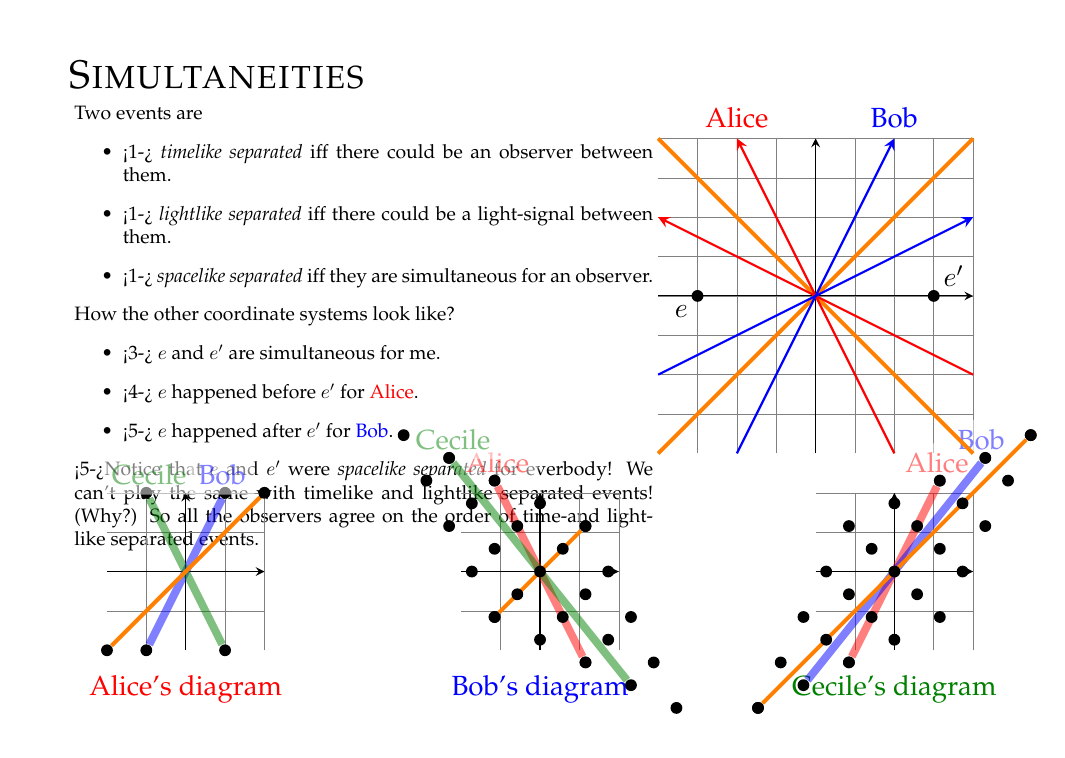
\begin{tikzpicture}[>=stealth, scale=1,
world/.style={inner sep=0, minimum size=.15cm, fill=black, circle},
worldline/.style={line width=1mm, rounded corners=1pt, opacity=.5},
axis/.style={->},
light/.style={orange, line width=.5mm},
]
\pgfmathdeclarefunction{XLorentz}{3}{\pgfmathparse{(#2 - #1*#3)/(sqrt(1-(#1)^2))}} % speed, spacecoord, timecoord
\pgfmathdeclarefunction{YLorentz}{3}{\pgfmathparse{(#3 - #1*#2)/(sqrt(1-(#1)^2))}} % speed, spacecoord, timecoord

%%%%%%%%%%%%%%%%%%%%%%%% DIA KEZDETE %%%%%%%%%%%%%%%%%%%%%%%%%%%

\node[anchor=north west, inner sep=0] at (0.5,8.5) {\textsc{\Large Simultaneities}}; %%%%%%% TITLE
%\node[anchor=north west, inner sep=0] at (0.5,8) {\textsc{\normalsize Role of Light}}; %%%%%%% SUBTITLE
\draw[white]  %%%%%%%%%%%% SIZE OF THE SLIDE
      (0,0) rectangle (12.77,8.9);
%%%%%%%%% TEXT %%%%%%%%%%%%%
\node[anchor=north west, scale=.7] at (0.5,8) {\begin{minipage}{10.5cm}
Two events are \begin{itemize}
\item<1-> \emph{timelike separated} iff there could be an observer between them.
\item<1-> \emph{lightlike separated} iff there could be a light-signal between them.
\item<1-> \emph{spacelike separated} iff they are simultaneous for an observer.
\end{itemize}
How the other coordinate systems look like?
\begin{itemize}
\item<3-> $e$ and $e'$ are simultaneous for me.
\item<4-> $e$ happened before $e'$ for \textcolor{red}{Alice}.
\item<5-> $e$ happened after $e'$ for \textcolor{blue}{Bob}.
\end{itemize}
\uncover<5->{Notice that $e$ and $e'$ were \emph{spacelike separated} for everbody! We can't play the same with timelike and lightlike separated events! (Why?) So all the observers agree on the order of time-and lightlike separated events.}
\end{minipage}
};
%%%%%%%%%%%%%%%%%%%%%%%% KOORDINÁTARENDSZEREK %%%%%%%%%%%%%%%%%%%%%%%%%%%
\coordinate(O1) at (2,2) {} {};
  \CoordSys{O1}{1}{1}
\coordinate(O2) at (6.5,2) {} {};
  \CoordSys{O2}{1}{1}
\coordinate(O3) at (11,2) {} {} {};
  \CoordSys{O3}{1}{1}

\coordinate(O4) at (10,5.5) {} {} {} {} {};
  \CoordSys{O4}{2}{2}

%%%%%%%%%%%%%%%
%%% SETTINGS %%
%%%%%%%%%%%%%%%


\coordinate (SignalStart) at (1,1) {} {} {};
\coordinate (SignalBounced) at (3,3) {} {} {};
\coordinate (AliceStart) at (2,1) {} {} {};
\coordinate (AliceEnd) at (2,3) {} {} {};
\coordinate (BobStart) at (1.5,1) {} {} {} {} {} {}; % Fontos hogy átmenjen az Origón, különben rossz a lorentz transzformáció!!
\coordinate (BobEnd) at (2.5,3) {} {} {} {} {} {};
\coordinate(CecileEnd) at (1.5,3) {};
\coordinate(CecileStart) at (2.5,1) {};

%%%%%%%%%%% Ezt lehetne macronak, speedszámítócuccnak
\path (BobStart); \pgfgetlastxy{\XCoord}{\YCoord}; % Extracting coordinates of the Origin
\pgfmathsetmacro{\XFirst}{\XCoord} % Saving X coordinate
\pgfmathsetmacro{\YFirst}{\YCoord} % Saving Y coordinate
\path (BobEnd); \pgfgetlastxy{\XCoord}{\YCoord}; % Extracting coordinates of the Point
\pgfmathsetmacro{\XSecond}{\XCoord} % Saving X coordinate
\pgfmathsetmacro{\YSecond}{\YCoord} % Saving Y coordinate
\pgfmathsetmacro{\SpeedBob}{(\XFirst-\XSecond)/(\YFirst-\YSecond)} % Relativizing to the origin
%%%%%%%%%%%%%%%%%%%%%%%%%%%%%%%%%%%

\Lorentz{O1}{O1}{0}{BobStart}{BS}
\Lorentz{O1}{O1}{0}{BobEnd}{BE}
\Lorentz{O1}{O1}{0}{CecileStart}{CS}
\Lorentz{O1}{O1}{0}{CecileEnd}{CE}
\Lorentz{O1}{O1}{0}{SignalStart}{SS}
\Lorentz{O1}{O1}{0}{SignalBounced}{SB}
\Lorentz{O1}{O2}{\SpeedBob}{AliceStart}{AS'}
\Lorentz{O1}{O2}{\SpeedBob}{AliceEnd}{AE'}
\Lorentz{O1}{O2}{\SpeedBob}{CecileStart}{CS'}
\Lorentz{O1}{O2}{\SpeedBob}{CecileEnd}{CE'}
\Lorentz{O1}{O2}{\SpeedBob}{SignalStart}{SS'}
\Lorentz{O1}{O2}{\SpeedBob}{SignalBounced}{SB'}
\Lorentz{O1}{O3}{-\SpeedBob}{AliceStart}{AS''}
\Lorentz{O1}{O3}{-\SpeedBob}{AliceEnd}{AE''}
\Lorentz{O1}{O3}{-\SpeedBob}{BobStart}{BS''}
\Lorentz{O1}{O3}{-\SpeedBob}{BobEnd}{BE''}
\Lorentz{O1}{O3}{-\SpeedBob}{SignalStart}{SS''}
\Lorentz{O1}{O3}{-\SpeedBob}{SignalBounced}{SB''}
\node[rotate=0, text=red, fill=white] at (2,0.5) {Alice's diagram};
\node[rotate=0, text=blue, fill=white] at (6.5,0.5) {Bob's diagram};
\node[rotate=0, text=green!50!black, fill=white] at (11,0.5) {Cecile's diagram};
\draw[worldline, blue] (BS)--(BE) node[fill=white, above, pos=1]{Bob};
\draw[worldline, green!50!black] (CS)--(CE) node[fill=white, above, pos=1]{Cecile};
\draw[worldline, red] (AS')--(AE') node[fill=white, above, pos=1]{Alice};
\draw[worldline, green!50!black] (CS')--(CE') node[fill=white, above, pos=1]{Cecile};
\draw[worldline, red] (AS'')--(AE'') node[fill=white, above, pos=1]{Alice};
\draw[worldline, blue] (BS'')--(BE'') node[fill=white, above, pos=1]{Bob};
\draw[light]  (SS)   -- (SB);
\draw[light]  (SS')  -- (SB');
\draw[light]  (SS'') -- (SB'');

\pause

\foreach \x in {1, 1.5, ..., 3}
{\foreach \y in {1, 1.5, ..., 3}
 { %\coordinate(\x\y) at (\x,\y);
   \Lorentz{O1}{O2}{\SpeedBob}{\x,\y}{}
   \Lorentz{O1}{O3}{-\SpeedBob}{\x,\y}{}
 }}

\pause

\coordinate (v1) at (10.5,7.5) {} {};
\coordinate (v2) at (12,6) {} {};
\coordinate (v3) at (11,7.5) {} {};
\coordinate (v4) at (12,6.5) {} {};
\coordinate (v5) at (11.5,7.5) {} {};
\coordinate (v6) at (12,7) {} {};
\coordinate (v7) at (9.5,3.5) {} {};
\coordinate (v8) at (8,5) {} {};
\coordinate (v9) at (9,3.5) {} {};
\coordinate (v10) at (8,4.5) {} {};
\coordinate (v11) at (8.5,3.5) {} {};
\coordinate (v12) at (8,4) {} {};
\coordinate (v15) at (12,5) {} {};
\coordinate (v13) at (10.5,3.5) {} {};
\coordinate (v19) at (12,4.5) {} {};
\coordinate (v17) at (11,3.5) {} {};
\coordinate (v23) at (12,4) {} {};
\coordinate (v21) at (11.5,3.5) {} {};
\coordinate (v14) at (9.5,7.5) {} {};
\coordinate (v16) at (8,6) {} {};
\coordinate (v18) at (9,7.5) {} {};
\coordinate (v20) at (8,6.5) {} {};
\coordinate (v22) at (8.5,7.5) {} {};
\coordinate (v24) at (8,7) {} {};
\coordinate (v25) at (8,3.5) {} {} {};
\coordinate (v26) at (12,7.5) {} {} {};
\coordinate (v28) at (8,7.5) {} {} {};
\coordinate (v27) at (12,3.5) {} {} {};
\draw[light]  (v25) edge (v26);
\draw[light]  (v27) edge (v28);
\node[world](e) at (8.5,5.5) {};
\node[anchor=north east] at (e){$e$};
\node[world](e') at (11.5,5.5) {};
\node[anchor=south west] at (e'){$e'$};
\begin{scope}[->, thick]
\pause
\draw[red]  (v17) -- (v18);
\draw[red]  (v19) -- (v20);
\node[red, anchor=south] at (v18) {Alice};
\pause
\draw[blue]  (v9) -- (v3);
\draw[blue]  (v10) -- (v4);
\node[blue, anchor=south] at (v3) {Bob};
%\pause
%\draw[gray]  (v21) -- (v22);
%\draw[gray]  (v23) -- (v24);
%\node[gray, anchor=west, rotate=90] at (v22) {Cecile};
%\pause
%\draw[violet]  (v13) -- (v14);
%\draw[violet]  (v15) -- (v16);
%\node[violet, anchor=west, rotate=90] at (v14) {Daniel};
%\pause
%\draw[green!50!black]  (v11) -- (v5);
%\draw[green!50!black]  (v12) -- (v6);
%\node[green!50!black, anchor=west, rotate=90] at (v5) {Elliot};
%\pause
%\draw[brown]  (v7) -- (v1);
%\draw[brown]  (v8) -- (v2);
%\node[brown, anchor=west, rotate=90] at (v1) {Fay};
\end{scope}
\end{tikzpicture}
\]
\end{frame}
%%%%%%%%%%%%%%%%%%%%%%%%%% SLIDE %%%%%%%%%%%%%%%%%%%%%%%%%%


\begin{frame}[fragile]
\vspace{-.55cm}
\[
\hspace{-1cm}
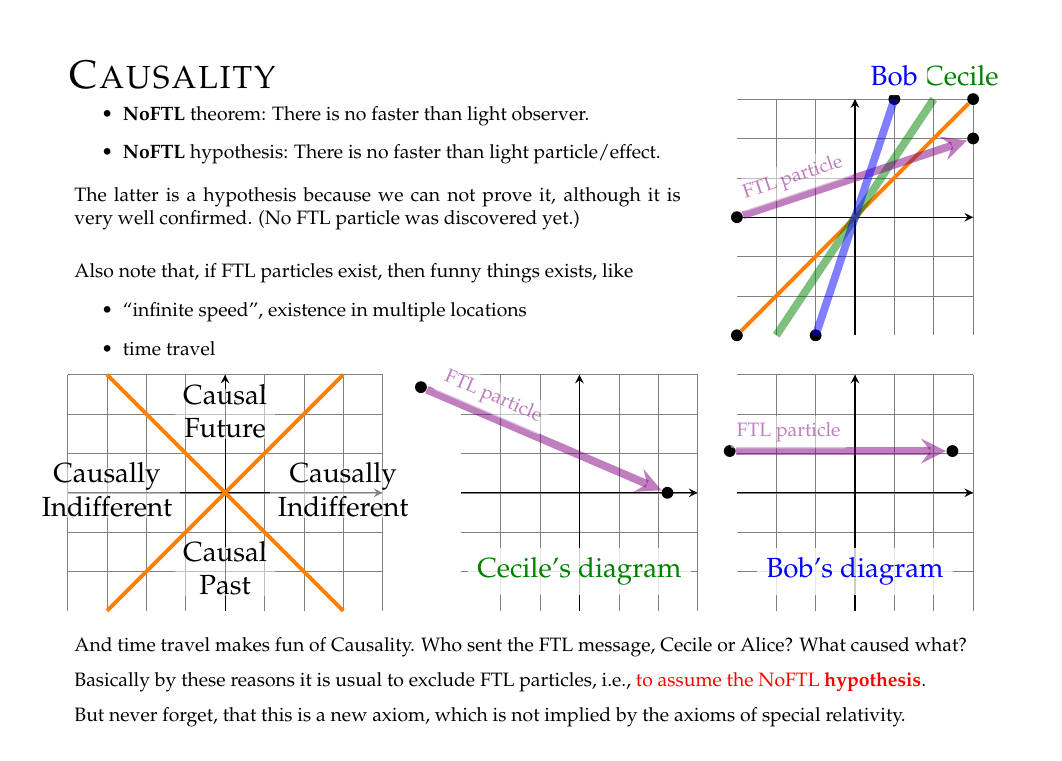
\begin{tikzpicture}[>=stealth, scale=1,
world/.style={inner sep=0, minimum size=.15cm, fill=black, circle},
worldline/.style={line width=1mm, rounded corners=1pt, opacity=.5},
axis/.style={->},
light/.style={orange, line width=.5mm},
]
\pgfmathdeclarefunction{XLorentz}{3}{\pgfmathparse{(#2 - #1*#3)/(sqrt(1-(#1)^2))}} % speed, spacecoord, timecoord
\pgfmathdeclarefunction{YLorentz}{3}{\pgfmathparse{(#3 - #1*#2)/(sqrt(1-(#1)^2))}} % speed, spacecoord, timecoord

%%%%%%%%%%%%%%%%%%%%%%%% DIA KEZDETE %%%%%%%%%%%%%%%%%%%%%%%%%%%

\node[anchor=north west, inner sep=0] at (0.5,8.5) {\textsc{\Large Causality}}; %%%%%%% TITLE
\draw[white]  %%%%%%%%%%%% SIZE OF THE SLIDE
      (0,0) rectangle (12.77,8.9);
%%%%%%%%% TEXT %%%%%%%%%%%%%
\node[anchor=north west, scale=.7] at (0.5,8) {\begin{minipage}{11cm}
\begin{itemize}
\item \textbf{NoFTL} theorem: There is no faster than light observer.
\item \textbf{NoFTL} hypothesis: There is no faster than light particle/effect.
\end{itemize}
The latter is a hypothesis because we can not prove it, although it is very well confirmed. (No FTL particle was discovered yet.)
\end{minipage}
};
%%%%%%%%%%%%%%%%%%%%%%%% KOORDINÁTARENDSZEREK %%%%%%%%%%%%%%%%%%%%%%%%%%%

%%%%%%%%%%
%% SETTINGS %%
%%%%%%%%%%

\coordinate (SignalStart) at (9,5) {} {} {} {} {};
\coordinate (SignalBounced) at (12,8) {} {} {} {};
\coordinate (AliceStart) at (10.5,5) {} {} {} {};
\coordinate (AliceEnd) at (10.5,8) {} {} {} {};
\coordinate (BobStart) at (10,5) {} {} {} {} {} {} {}; % Fontos hogy átmenjen az Origón, különben rossz a lorentz transzformáció!!
\coordinate (BobEnd) at (11,8) {} {} {} {} {} {} {};
\coordinate (CecileStart) at (9.5,5) {} {} {} {} {} {} {} {}; % Fontos hogy átmenjen az Origón, különben rossz a lorentz transzformáció!!
\coordinate (CecileEnd) at (11.5,8) {} {} {} {} {} {} {} {};
\coordinate(FTLStart) at (9,6.5) {} {};
\coordinate(FTLEnd) at (12,7.5) {} {};

%%%%%%%%%%% Ezt lehetne macronak, speedszámítócuccnak
\path (BobStart); \pgfgetlastxy{\XCoord}{\YCoord}; % Extracting coordinates of the Origin
\pgfmathsetmacro{\XFirst}{\XCoord} % Saving X coordinate
\pgfmathsetmacro{\YFirst}{\YCoord} % Saving Y coordinate
\path (BobEnd); \pgfgetlastxy{\XCoord}{\YCoord}; % Extracting coordinates of the Point
\pgfmathsetmacro{\XSecond}{\XCoord} % Saving X coordinate
\pgfmathsetmacro{\YSecond}{\YCoord} % Saving Y coordinate
\pgfmathsetmacro{\SpeedBob}{(\XFirst-\XSecond)/(\YFirst-\YSecond)} % Relativizing to the origin
%%%%%%%%%%%%%%%%%%%%%%%%%%%%%%%%%%%
%%%%%%%%%%% Ezt lehetne macronak, speedszámítócuccnak
\path (CecileStart); \pgfgetlastxy{\XCoord}{\YCoord}; % Extracting coordinates of the Origin
\pgfmathsetmacro{\XFirst}{\XCoord} % Saving X coordinate
\pgfmathsetmacro{\YFirst}{\YCoord} % Saving Y coordinate
\path (CecileEnd); \pgfgetlastxy{\XCoord}{\YCoord}; % Extracting coordinates of the Point
\pgfmathsetmacro{\XSecond}{\XCoord} % Saving X coordinate
\pgfmathsetmacro{\YSecond}{\YCoord} % Saving Y coordinate
\pgfmathsetmacro{\SpeedCecile}{(\XFirst-\XSecond)/(\YFirst-\YSecond)} % Relativizing to the origin
%%%%%%%%%%%%%%%%%%%%%%%%%%%%%%%%%%%

 \pause

\coordinate(O1) at (10.5,6.5) {} {};
  \CoordSys{O1}{1.5}{1.5}

\Lorentz{O1}{O1}{0}{BobStart}{BS}
\Lorentz{O1}{O1}{0}{BobEnd}{BE}
\Lorentz{O1}{O1}{0}{SignalStart}{SS}
\Lorentz{O1}{O1}{0}{SignalBounced}{SB}
\Lorentz{O1}{O1}{0}{FTLStart}{FTLS}
\Lorentz{O1}{O1}{0}{FTLEnd}{FTLE}
\coordinate(O2) at (10.5,3) {} {} {};
  \CoordSys{O2}{1.5}{1.5}
\coordinate(O3) at (7,3) {} {} {} {};
  \CoordSys{O3}{1.5}{1.5}
\Lorentz{O1}{O2}{\SpeedBob}{FTLStart}{FTLS'}
\Lorentz{O1}{O2}{\SpeedBob}{FTLEnd}{FTLE'}
\Lorentz{O1}{O3}{\SpeedCecile}{FTLStart}{FTLS''}
\Lorentz{O1}{O3}{\SpeedCecile}{FTLEnd}{FTLE''}
\draw[light]  (SS)-- (SB);
\node[blue, fill=white, fill opacity=.8, text opacity=1] at (10.5,2) {Bob's diagram};
\node[green!50!black, fill=white, fill opacity=.8, text opacity=1] at (7,2) {Cecile's diagram};


\draw[worldline, green!50!black]  (CecileStart)-- (CecileEnd) node[above, fill opacity=1]{\qquad Cecile};
\draw[worldline, violet, ->]  (FTLS)-- (FTLE) node[above, pos=.25, fill=white, scale=.7, sloped]{FTL particle};
\draw[worldline, violet, ->]  (FTLS')-- (FTLE') node[above, pos=.25, fill=white, scale=.7, sloped]{FTL particle};
\draw[worldline, violet, ->]  (FTLS'')-- (FTLE'') node[above, pos=.25, fill=white, scale=.7, sloped]{FTL particle};
\draw[worldline, blue]  (BobStart)-- (BobEnd) node[above, pos=1, fill=white, fill opacity=1]{Bob};

\node[anchor=north west, scale=.7] at (0.5,6) {%
\begin{minipage}{12cm}
Also note that, if FTL particles exist, then funny things exists, like
\begin{itemize}
\item ``infinite speed'', existence in multiple locations
\item time travel
\end{itemize}
\end{minipage}};
\node[anchor=north west, scale=.7] at (0.5,1.25) {%
\begin{minipage}{17cm}
And time travel makes fun of Causality. Who sent the FTL message, Cecile or Alice? What caused what?

\medskip

Basically by these reasons it is usual to exclude FTL particles, i.e., \textcolor{red}{to assume the NoFTL \textbf{hypothesis}}.

\medskip

But never forget, that this is a new axiom, which is not implied by the axioms of special relativity.
\end{minipage}};

\pause

\coordinate(O4) at (2.5,3) {} {} {} {} {} {};
  \CoordSys{O4}{2}{1.5}


\coordinate (v4) at (1,1.5) {};
\coordinate (v3) at (4,4.5) {};
\coordinate (v1) at (1,4.5) {};
\coordinate (v2) at (4,1.5) {};
\draw[light]  (v1) edge (v2);
\draw[light]  (v3) edge (v4);
\node[inner sep=-3,fill=white, fill opacity=.5, text opacity=1] at (2.5,4) {\begin{tabular}{c}Causal \\ Future\end{tabular}};
\node[inner sep=-3,fill=white, fill opacity=.5, text opacity=1] at (2.5,2) {\begin{tabular}{c}Causal \\ Past\end{tabular}};
\node[inner sep=-3,fill=white, fill opacity=.5, text opacity=1] at (4,3) {\begin{tabular}{c}Causally \\ Indifferent\end{tabular}};
\node[inner sep=-3,fill=white, fill opacity=.5, text opacity=1] at (1,3) {\begin{tabular}{c}Causally \\ Indifferent\end{tabular}};
\end{tikzpicture}\]
\end{frame}

\szakasz[Minkowski distance]{Minkowski distance}
\begin{frame}[t]
\frametitle{Motivating Minkowski distance}
We are looking for an \emph{observer-independent} distance events.

\dzsa{Moral of paradigmatic effects} Observers may not agree on the spatial distance and elapsed time between events.

\dzsa{But} proper relativity needs non-zero relative speed. Parallel moving observers agree on elapsed time and spatial distance.

\dzsa{Idea} Every observer will have its own jurisdiction, and every observer has to ask the \cemph{competent} observer to decide Minkowski distance.

$k$ is \cemph{competent} for $e$ and $e'$ iff they are on the worldline of $k$ or they both happened when $k$'s clock showed $0$.
\[
\mu_k (e,e')\defegy
\left\{
\begin{array}{ll}
   x  & \textup{ if $m$ \emph{crosses} $e$ and $e'$ (they happen $0$ far away)} 
        \\ & \textup{ $x$ measures the elapsed time between $e$ and $e'$ to be $x$}
\\ 0  & \textup{ if there is a photon through $e$ and $e'$. (Everybody agree!)}
\\ -x & \textup{ if $m$ observes that $e$ and $e'$ happens at time 0}
        \\ & \textup{ and $m$ measures spatial distance between $e$ and $e'$ to be $x$.}
\end{array}
\right.
\]

Therefore this notion is observer-independent. Also, the Minkowski distance of $e$ and $e'$ according to $k$ happens to be
\[ \mu_k (e,e') = \sqrt{(e_t-e'_t)^2- (e_x-e'_x)^2- (e_y-e'_y)^2- (e_z-e'_z)^2} \]
where $e$ and $e'$ are coordinatized by $k$ on $(e_t, e_x, e_y, e_z)$ and $(e_t', e_x', e_y', e_z')$, respectively

\end{frame}

\begin{frame}[t]
\frametitle{$n$-dimensional Minkowski spacetime}
$n$ dimensional Minkowski spacetime is 
\[(\mathbb R^n, \mu)\]
where 
\[\mu(\vec x , \vec y) \defegy \sqrt{(\vec x_1 - \vec y_1)^2-\sum_{2\leq i\leq n} (\vec x_i - \vec y_i)^2 }\]
i.e., a spacetime diagram with its observer independent minkowski-distance.

\end{frame}
\end{document}
